\documentclass[a4paper]{report}

%====================== PACKAGES ======================

\usepackage[french]{babel}
\usepackage[utf8]{inputenc}
%pour gérer les positionnement d'images
\usepackage{float}
\usepackage{amsmath}
\usepackage{graphicx}
\usepackage[colorinlistoftodos]{todonotes}
\usepackage{url}
%pour les informations sur un document compilé en PDF et les liens externes / internes
\usepackage{hyperref}
\usepackage[final]{pdfpages}
%espacement entre les lignes
\usepackage{setspace}
%modifier la mise en page de l'abstract
\usepackage{abstract}
%police et mise en page (marges) du document
\usepackage[T1]{fontenc}
\usepackage[top=2cm, bottom=2cm, left=2cm, right=2cm]{geometry}
%Pour les galerie d'images
\usepackage{subfig}

%====================== INFORMATION ET REGLES ======================

%rajouter les numérotation pour les \paragraphe et \subparagraphe
\setcounter{secnumdepth}{4}
\setcounter{tocdepth}{4}

%======================== DEBUT DU DOCUMENT ========================

\begin{document}
\begin{spacing}{2}
\newcommand{\HRule}{\rule{\linewidth}{0.5mm}}
\begin{titlepage}
\begin{center}

% Upper part of the page. The '~' is needed because only works if a paragraph has started.

\includegraphics[width=0.35\textwidth]{./logo}~\\[1cm]

\textsc{\LARGE École nationale supérieure d'informatique et d'analyse des systèmes}\\[1.5cm]

\textsc{\Large }\\[0.5cm]

% Title
\HRule \\[0.4cm]

{\huge \bfseries Projet Ingénieurie Web et Développement\\
Application Web sur le covoiturage \\[0.4cm] }

\HRule \\[1.5cm]

% Author and supervisor
\begin{minipage}{0.4\textwidth}
\begin{flushleft} \large
\emph{Réalisé par:}\\
\textsc{BARKANI Ismail}\\
\textsc{BOUFOUS Abdellah}\\
\textsc{BOUZIANE Ilyas}\\
\end{flushleft}
\end{minipage}
\begin{minipage}{0.4\textwidth}
\begin{flushright} \large
\emph{Encadré par:} \\
Pr. \textsc{MAHMOUD\\EL HAMLAOUI}\\
\end{flushright}
\end{minipage}

\vfill

% Bottom of the page
{\large Année universitaire : 2019 - 2020}

\end{center}
\end{titlepage}

%page blanche
\newpage
\thispagestyle{empty}
~
\newpage
\thispagestyle{empty}
\tableofcontents
\thispagestyle{empty}
\listoffigures
\thispagestyle{empty}
\setcounter{page}{0}
%ne pas numéroter le sommaire

\newpage

%espacement entre les lignes d'un tableau
\renewcommand{\arraystretch}{1}

%====================== INCLUSION DES PARTIES ======================






\chapter*{Remerciements}
\addcontentsline{toc}{chapter}{Remerciements}

Avant tout développement sur ce projet, nous tenons à remercier du fond du cœur notre cher professeur monsieur EL HAMLAOUI Mahmoud qui nous a forme et accompagné  tout au long de notre travail avec beaucoup de patience et de pédagogie.

Un merci bien particulier adressé également à nos professeurs pour leurs remarques, leurs directives et l'intérêt qu'ils portent aux étudiants. Nous les remercions sincèrement pour leur suivi et leur orientation.


\chapter{Présentation du projet}
\section{Amenant}

\par 
Au cours de notre formation en tant qu'Elève Ingénieur de l'ENSIAS en 2ème année, nous sommes appelés à travailler sur un projet Java EE à travers lequel nous exploitons nos connaisances et compétences acquis durant notre formation \textbf{Développement et Ingéniere Web} afin d'aboutir à une application Web basé complètement sur Java EE bien construite. 

Avec l'accord de notre cher encadrant, nous avons choisi \textbf{Le covoiturage} comme sujet du projet. 

\section{Analyse de l'existant}

\par 
Face à la défaillance du système de transport ,le parc automobile marocain croît tous les ans avec son lot de désagréments: embouteillages, pollution, accident de la route sans oublier le stress des conducteurs. Le covoiturage pourrait être la solution à tous ces soucis en réduisant le trafic, et en diminuant la pollution ainsi que la consommation d’énergie.

Ainsi au Maroc, Plusieurs aujourd'hui optent pour cette alternative. Pour pallier aux problèmes liés à l’insuffisance de l’offre en matière du transport, à l’intérieur ou l’extérieur des villes, les Marocains prennent leurs maux en patience et innovent. Au sein des villes marocaines, face à l’anarchie régnante au sein du secteur du transport, le champ reste libre à plusieurs pratiques illégales dirigées par des \textit{"khattafas"}.

Alors que cette activité, pourtant punissable par la loi, tisse sa toile dans de nombreuses villes, toutes catégories confondues, le transport interrégional et entre les villes connait, lui aussi, un nouvel arrivant. Après des débuts timides sur le marché marocain, le covoiturage est devenu tendance, surtout chez les plus jeunes. Largement différent de l'auto-stop classique, le covoiturage consiste à partager les frais d’un trajet entre différentes personnes ; l’une d’elles étant un conducteur non professionnel disposant d’une voiture automobile.

Au Maroc, avec l’émergence des réseaux sociaux ,les groupes Facebook destinés à ce nouveau mode de transport se sont multipliés ces dernières années. Des centaines d’offres et de demandes sont publiées quotidiennement par les internautes, démontrant ainsi un réel engouement envers ce mode de transport destiné à pallier aux retards des trains, manque des moyens pour se procurer une voiture ou encore l’absence de confort de certains autocars.


\section{Problématique soulevée}
\par 
Le covoiturage n’est pas sans mésaventure. Mis à part son caractère illégal, le covoiturage au Maroc échappe à toute surveillance. Bien que les imposteurs sont régulièrement dénoncés par les utilisateurs et les administrateurs de ces groupes facebook, voyager avec un groupe d’inconnus au Maroc reste encore, pour plusieurs, un pas qui nécessite vigilance et réflexion préalable : Pour eux, le covoiturage c'est \textsf{Plus de peur que de mal}.

\par 
Par conséquent, deux problèmes majeurs trouvent chemin concernant le covoiturage au Maroc :
\begin{itemize}
\item[•] \textbf{La sécurité :} Que ce soient des applications comme Kareem ou sur des groupes Facebook, personne n'assure la sécurité des personnes transportés étant donné qu'ils sont d'origine illégale. 
\item[•] \textbf{L'organisation :} Toute personne souhaitant proposer ou demander un trajet sur des groupes Facebook dépose sa proposition ou sa demande sans avoir une connaissance préalable sur le conducteur ou encore sur le trajet exacte qu'il va prendre. De même, le conducteur a besoin d'avoir plus d'informations sur les personnes à prendre.                 
\end{itemize}
\cleardoublepage
\section{Solution proposée}

De ce qui précède, nous nous sommes aperçus que le besoin du covoiturage au Maroc, étant un besoin nécessaire et important, est à saisir et mérite une profonde réflexion aux problèmes cités avant. Ainsi, nous l'avons associé à notre projet JEE pour aboutir une application Web que nous avons nommé \textit{"Wessalani"} dont les objectifs sont :


\begin{itemize}
\item Assurer le covoiturage : mettre en relation des conducteurs voyageant avec des places libres et des passagers se rendant dans la même direction. Ils partagent un trajet et les frais qui y sont liés.
\item Assurer la sécurité des passagers et du conducteur : création d'un système interne au processus des choix et des propositions d'offres qui va permettre de donner plus de confiance à tous les partis et d'organiser un trajet en toute sécurité 
\item Assure l'organisation : établir une app Web intuitive qui va interagir avec le visiteur en toute simplicité sans avoir à parcourir plusieurs pages, seulement avec quelques cliques ou quelques messages au Chat Bot de l'application, et créer un sous-réseau social, géré par un/des administrateurs,
pour identifier les profils conducteurs afin de renforcer la sécurité 
\end{itemize}


\chapter{Analyse et Conception}

\par
La méthode que nous avons adopté pour réaliser l'analyse et la conception de
notre système d'information est la méthode UML : Elle permet la séparation
entre les données et les traitements effectuer en plusieurs modèles conceptuelles
qui sont répartis sur 3 diagrammes : Le diagramme de cas d’utilisation, le 
diagramme de classe, diagramme de séquence. Dans cette partie, nous allons 
présenter quelques-unes de ces méthodes, et en finissant par les maquettes.
Cette phase a pour objectif de déduire la spécication de l'architecture du système.

\section{Diagramme de cas d’utilisations}

les diagrammes de cas d'utilisation modélisent le comportement d'un système et permettent de capturer les exigences du système. Les diagrammes de cas d'utilisation décrivent
les fonctions générales et la portée d'un système. Ces diagrammes identifient également les
interactions entre le système et ses acteurs. Les cas d'utilisation et les acteurs dans les diagrammes de cas d'utilisation décrivent ce que le système fait et comment les acteurs l'utilisent,
mais ne montrent pas comment le système fonctionne en interne.
\cleardoublepage
\begin{itemize}
\item Diagramme de cas d’utilisation admin :
\begin{figure}[!ht]
\begin{center}
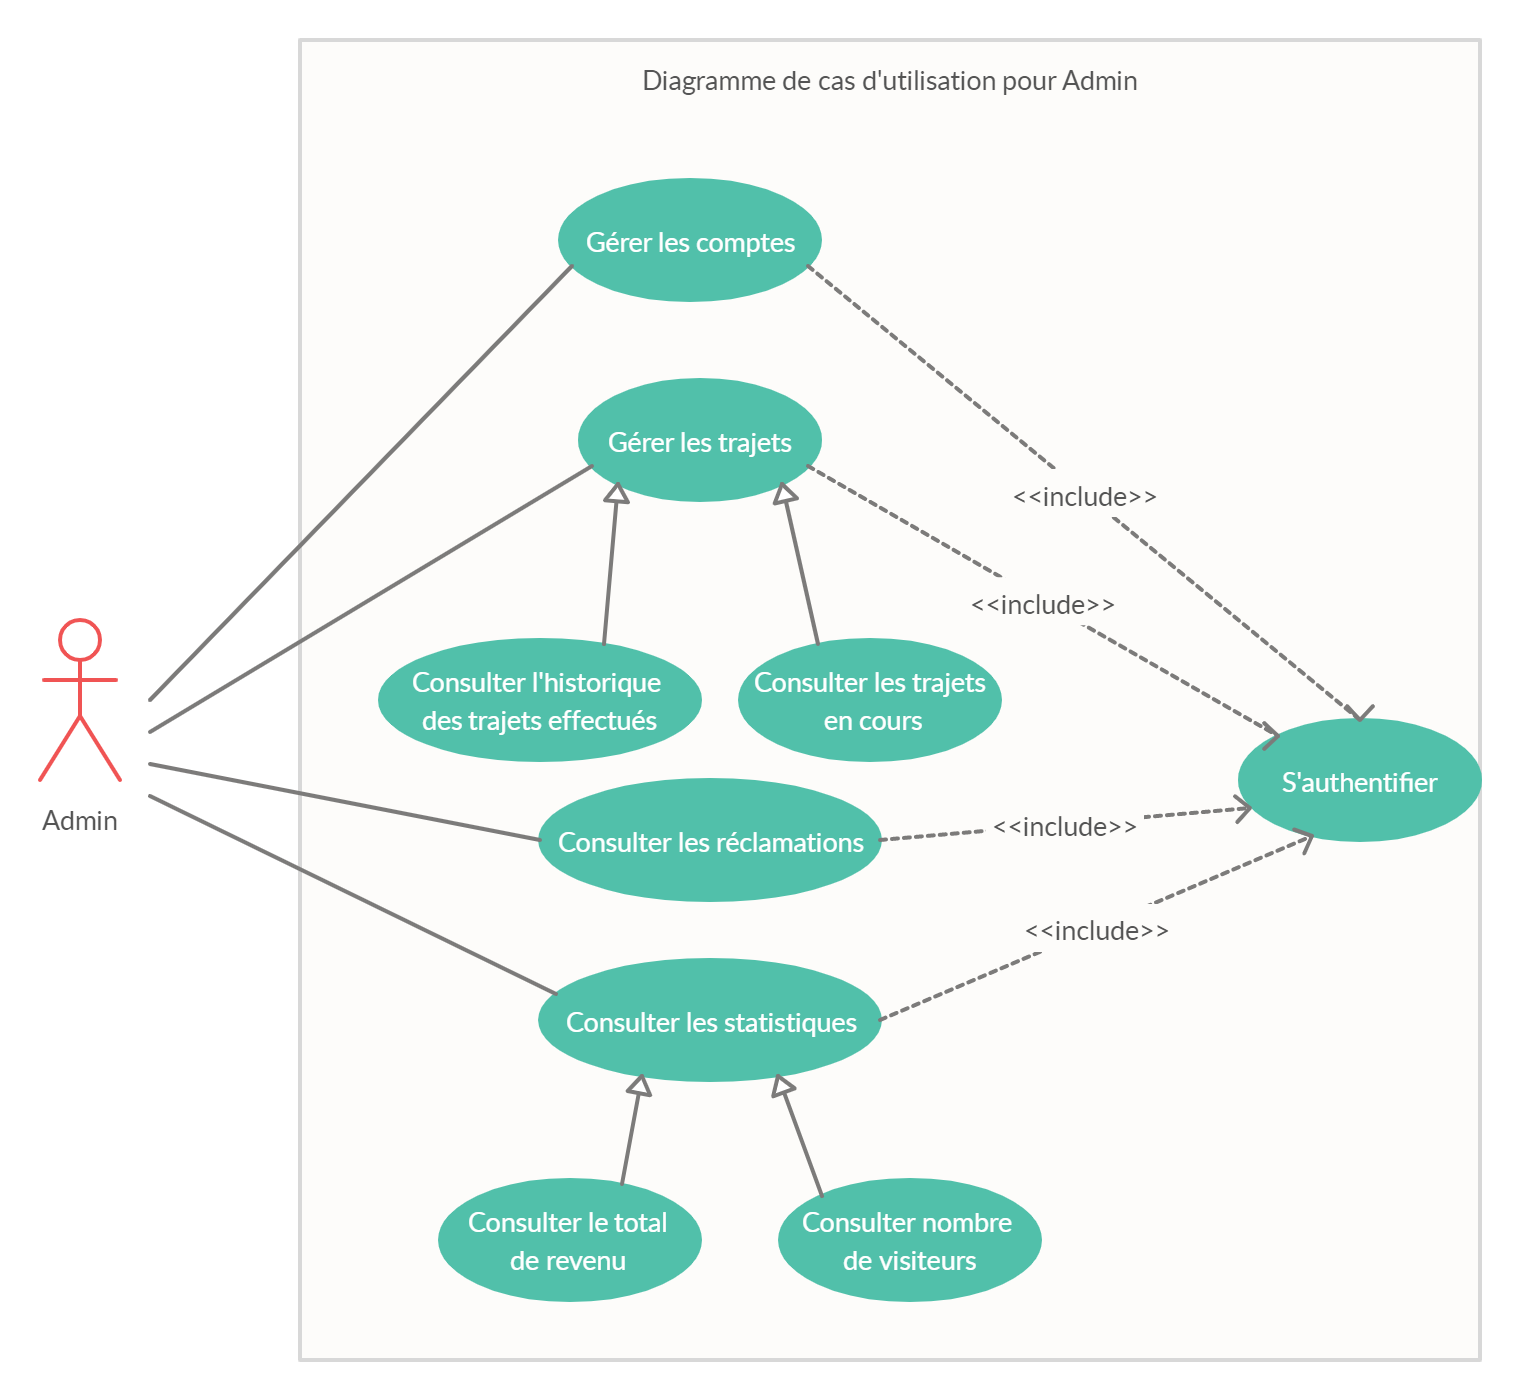
\includegraphics[height=8cm]{Projet_JEE/AdminUC.jpg}
\end{center}
\caption[Admin UC]{Admin UC}
\end{figure}
\cleardoublepage
\item Diagramme de cas d’utilisation utilisateur :
\begin{figure}[!ht]
\begin{center}
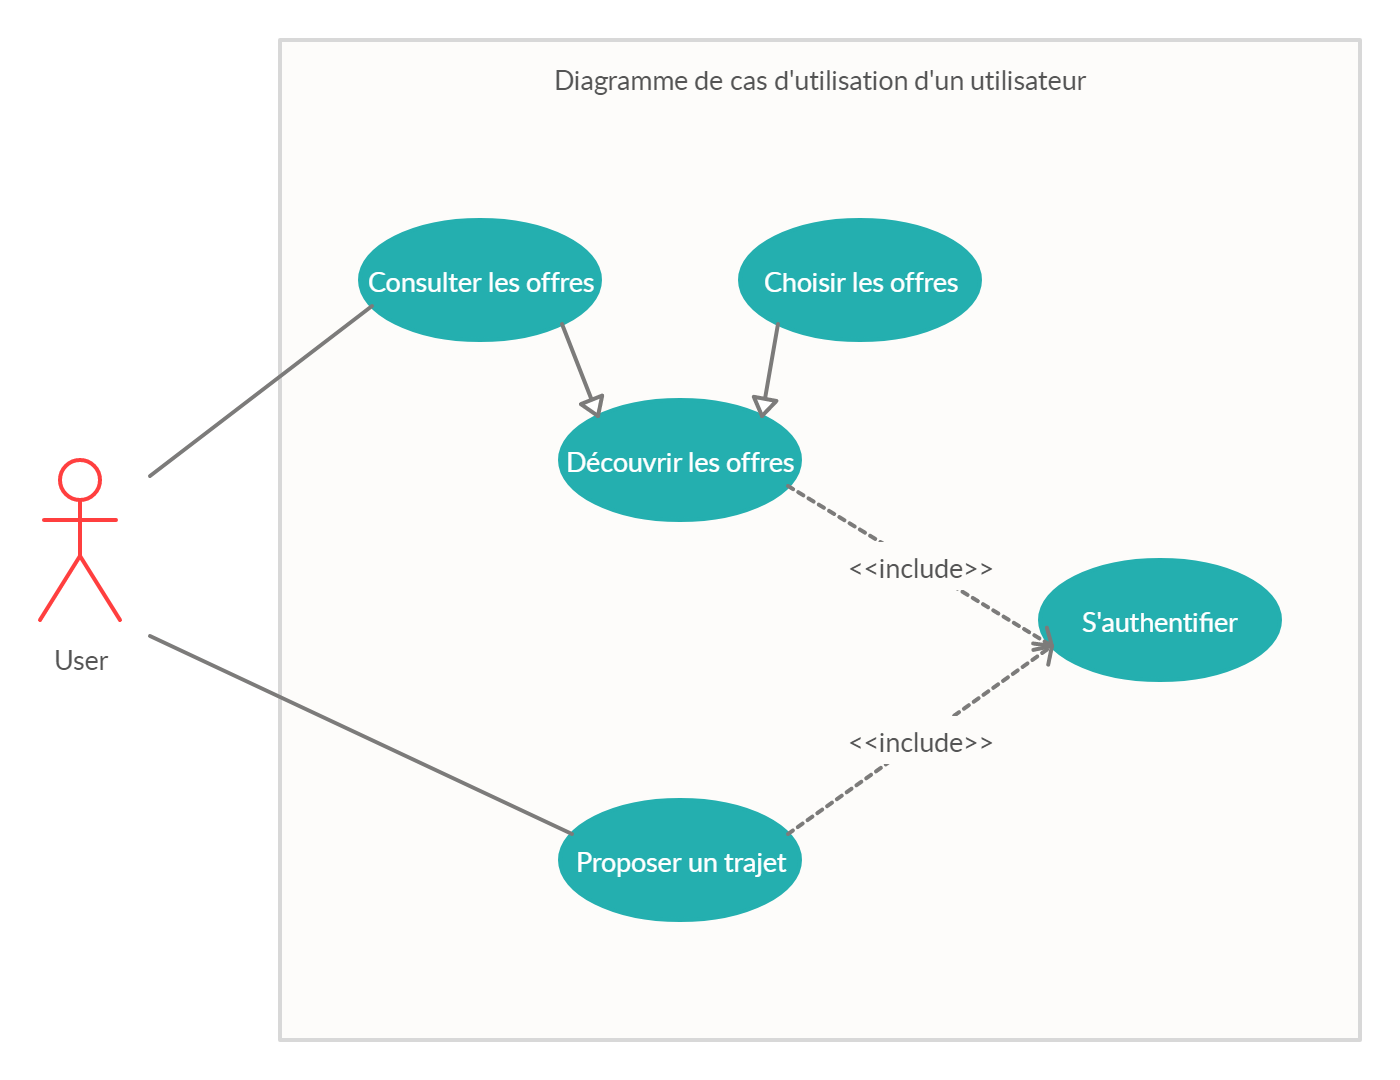
\includegraphics[height=8cm]{Projet_JEE/UserUC.jpg}
\end{center}
\caption[User UC]{User UC}
\end{figure}
 \cleardoublepage
\item Diagramme de cas d’utilisation visiteur :
\begin{figure}[!ht]
\begin{center}
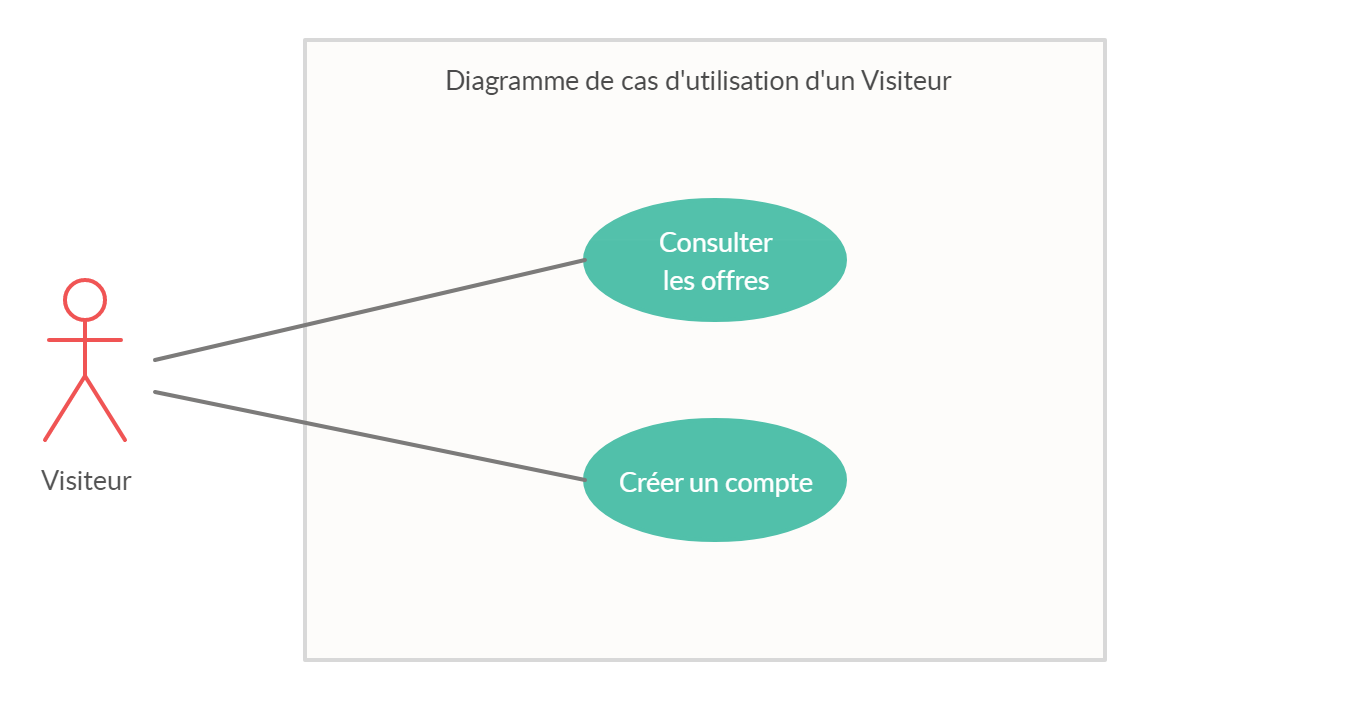
\includegraphics[height=8cm]{Projet_JEE/VisiteurUC.png}
\end{center}
\caption[Visiteur UC]{Visiteur UC}
\end{figure}
\cleardoublepage
 
\end{itemize}

\section{Diagramme de classe}
\begin{figure}[!ht]
\begin{center}
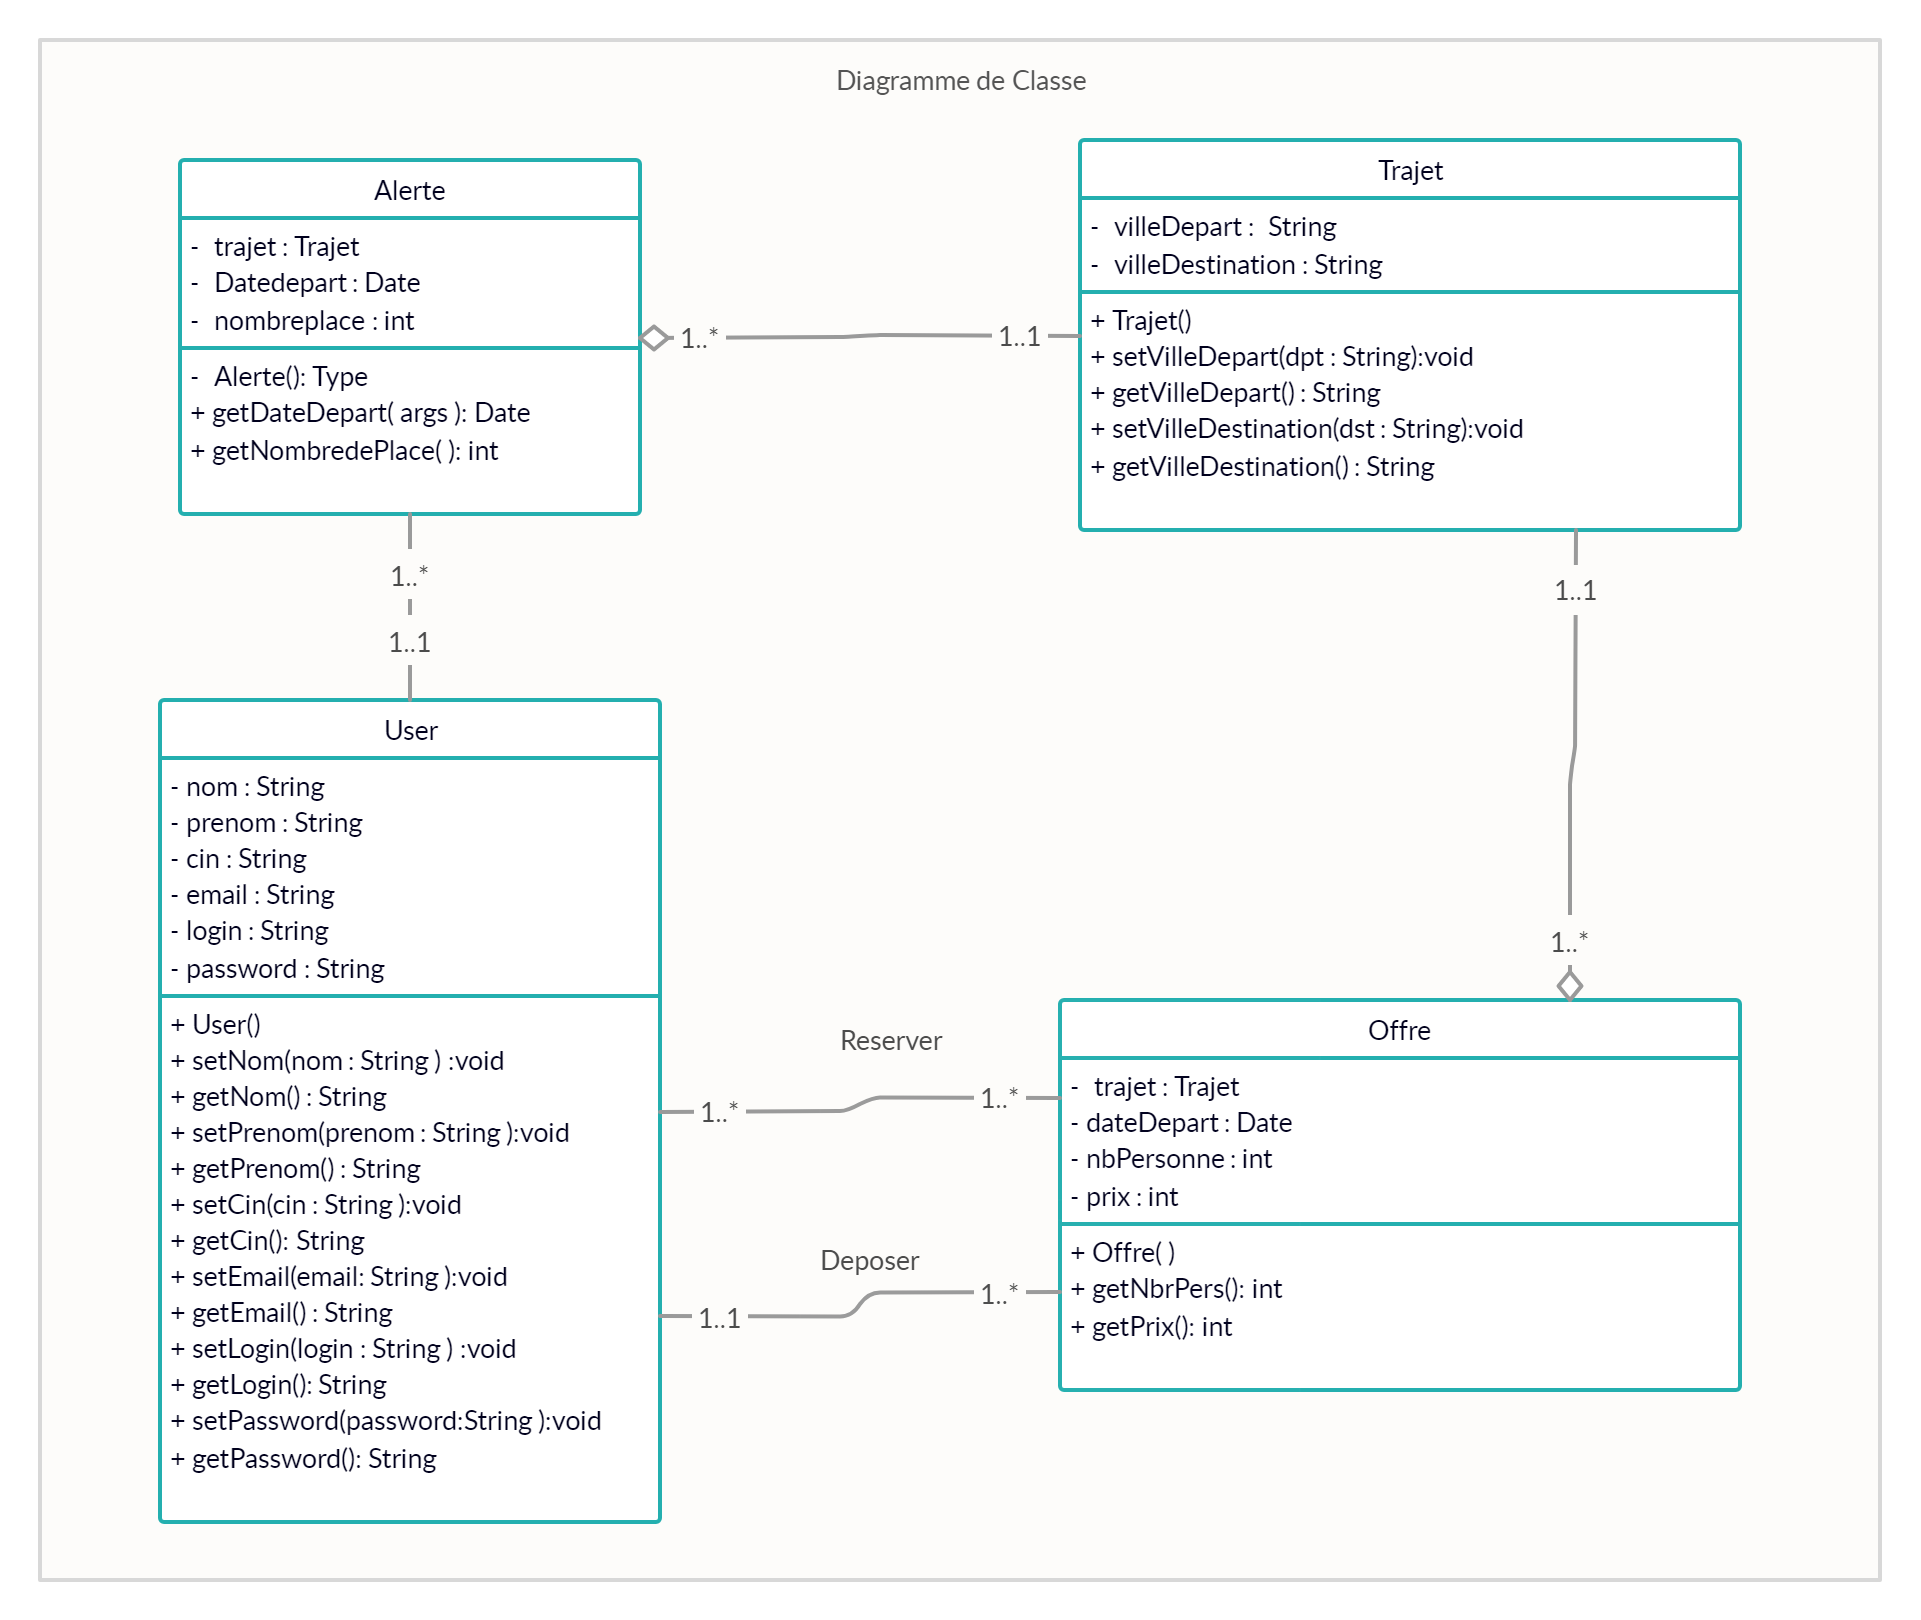
\includegraphics[height=10cm]{Projet_JEE/Diagramme de Classe.jpg}
\end{center}
\caption[Diagramme de classes]{Diagramme de classes}
\end{figure}
 
\section{Diagramme de séquences}
Pour schématiser la vue comportementale de notre système informatique, nous faisons recours au diagramme de séquence d'UML. Ce diagramme permet de présenter les interactions
entre l'acteur et le système avec des messages présentés dans un ordre chronologique. Le
diagramme de séquences traite le système informatique comme étant une boite noire. Le
comportement du système est décrit de l'extérieur sans avoir d'idée sur la réalisation. Nous
pouvons, alors, constater que certains cas d'utilisation sont similaires, c'est pourquoi nous
avons choisi de traiter quelques exemples.
\cleardoublepage
\begin{itemize}
\item Diagramme de séquence proposer trajet :
\begin{figure}[!ht]
\begin{center}
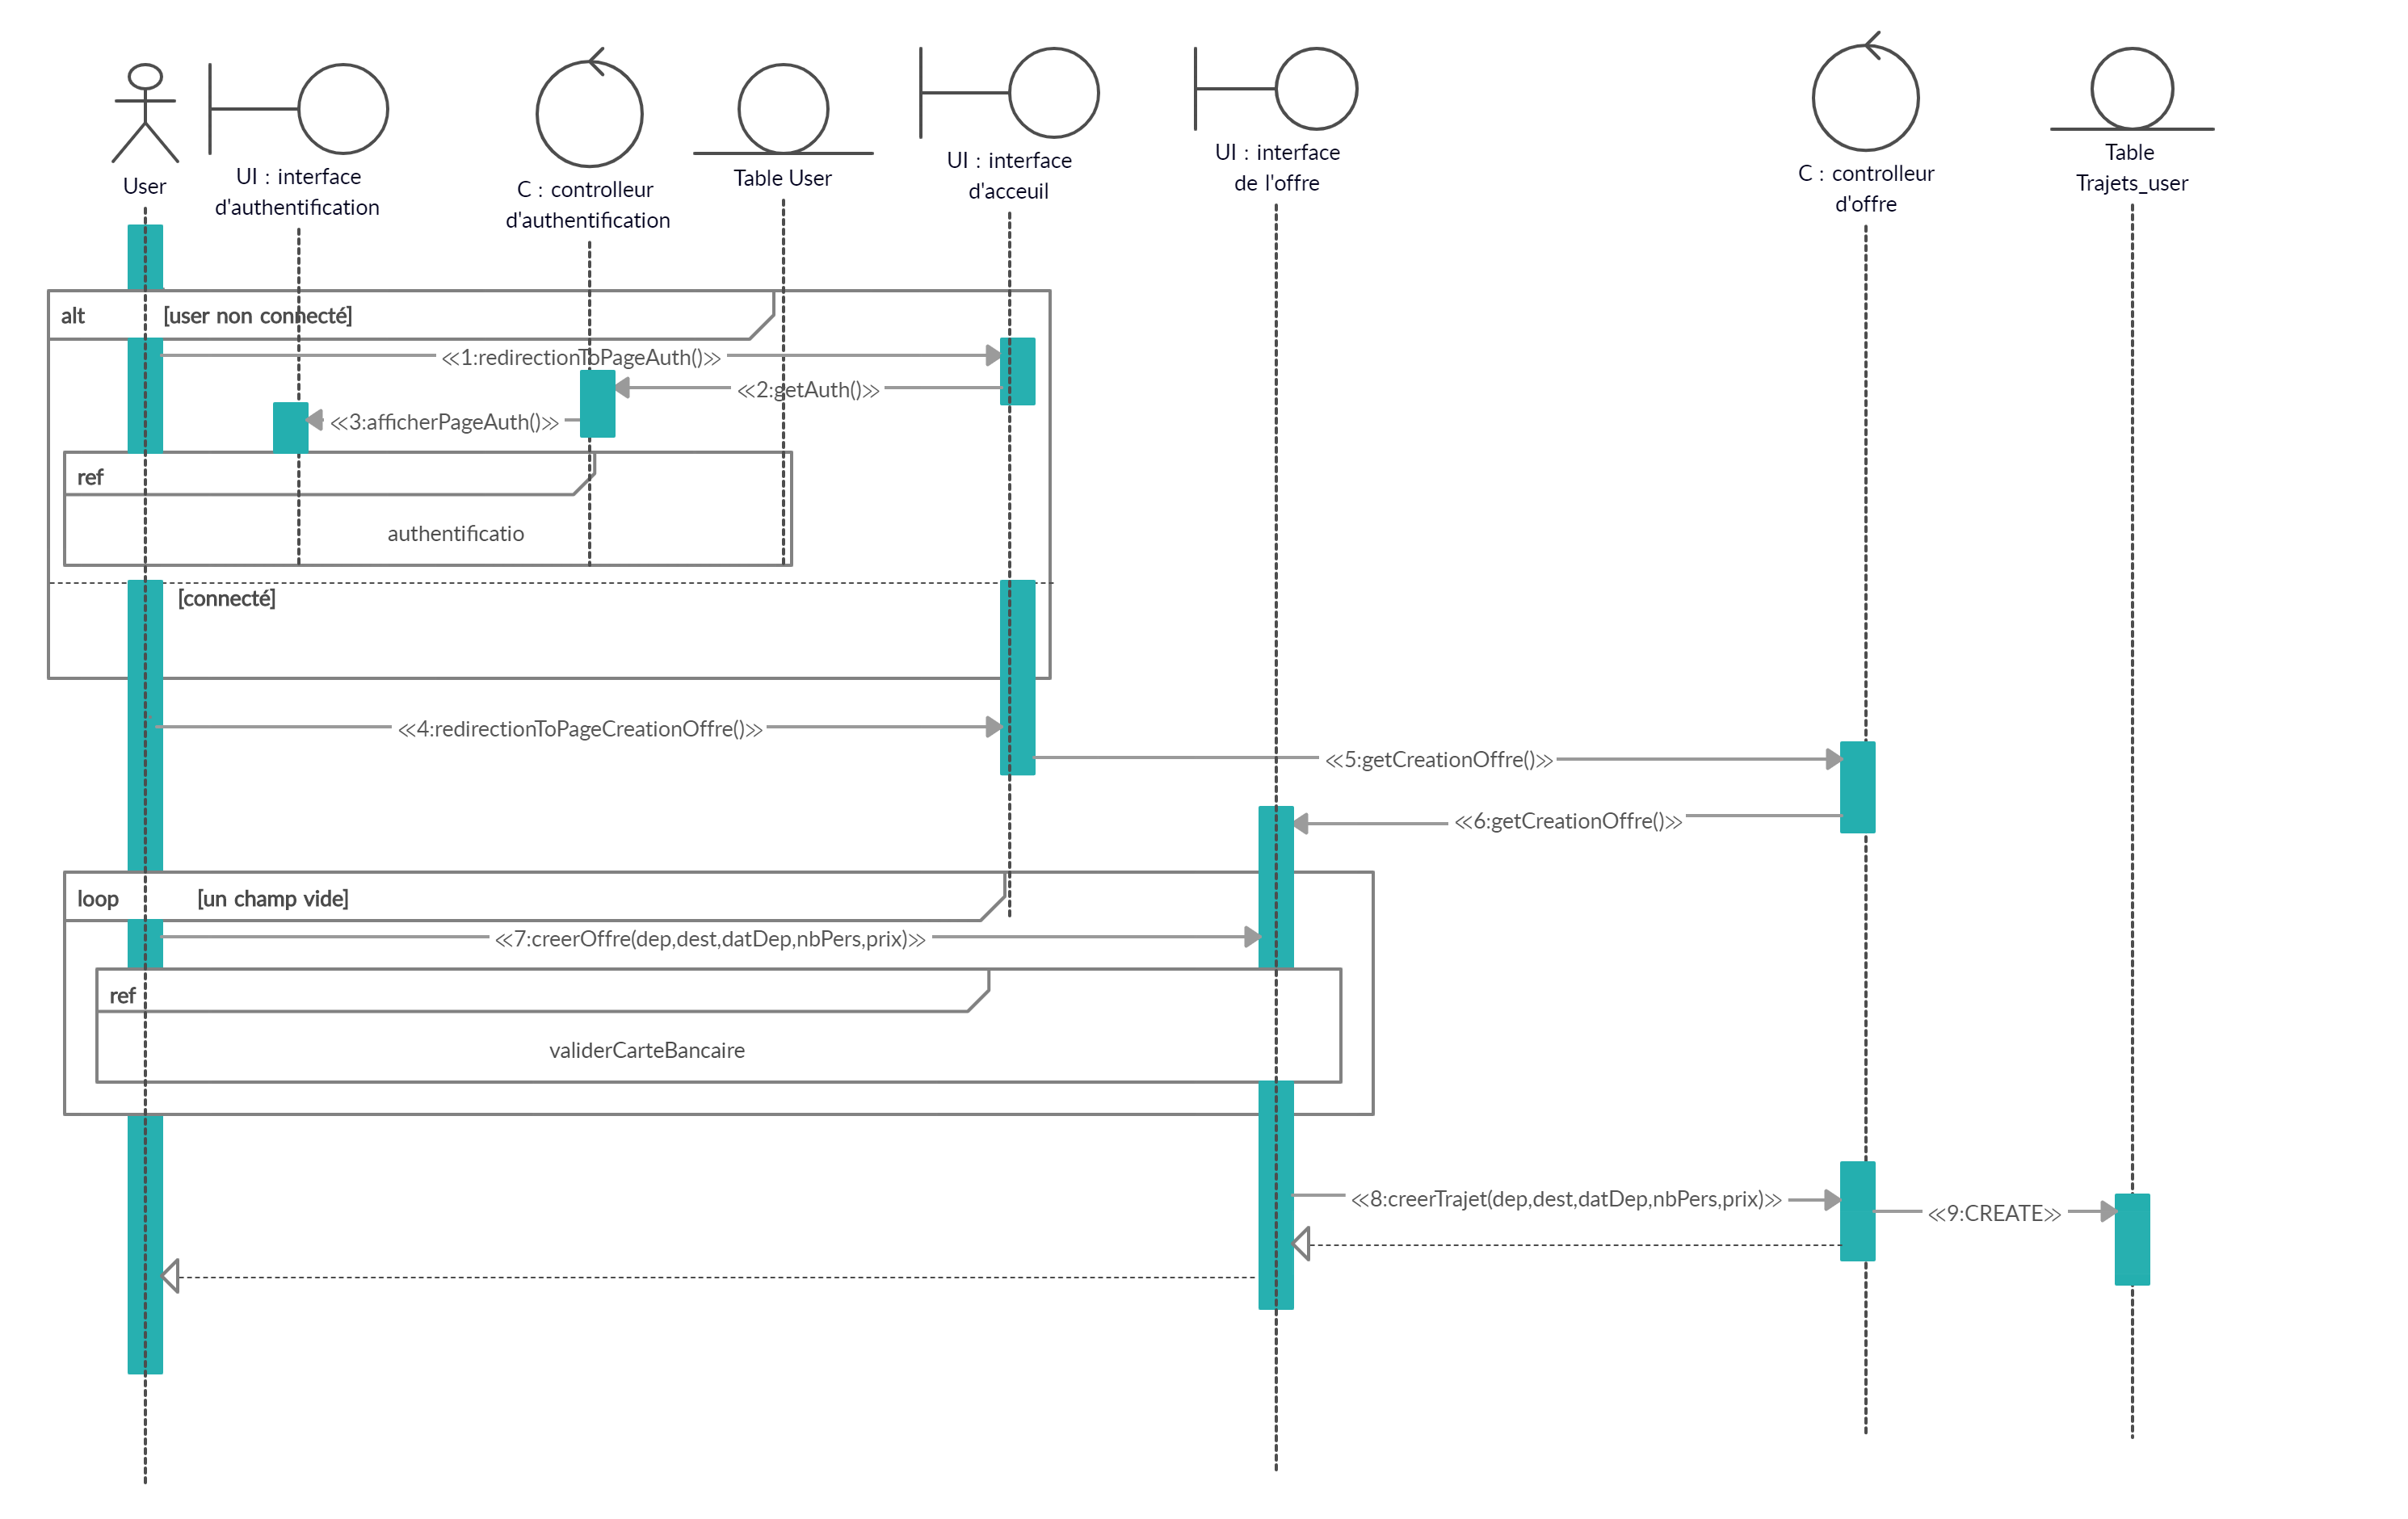
\includegraphics[angle=90,height=20cm]{Projet_JEE/SDproposerTrajet.jpg}
\end{center}
\caption[Proposer trajet]{Proposer trajet}
\end{figure}
\cleardoublepage
\item Diagramme de séquence consulter les offres :
\begin{figure}[!ht]
\begin{center}
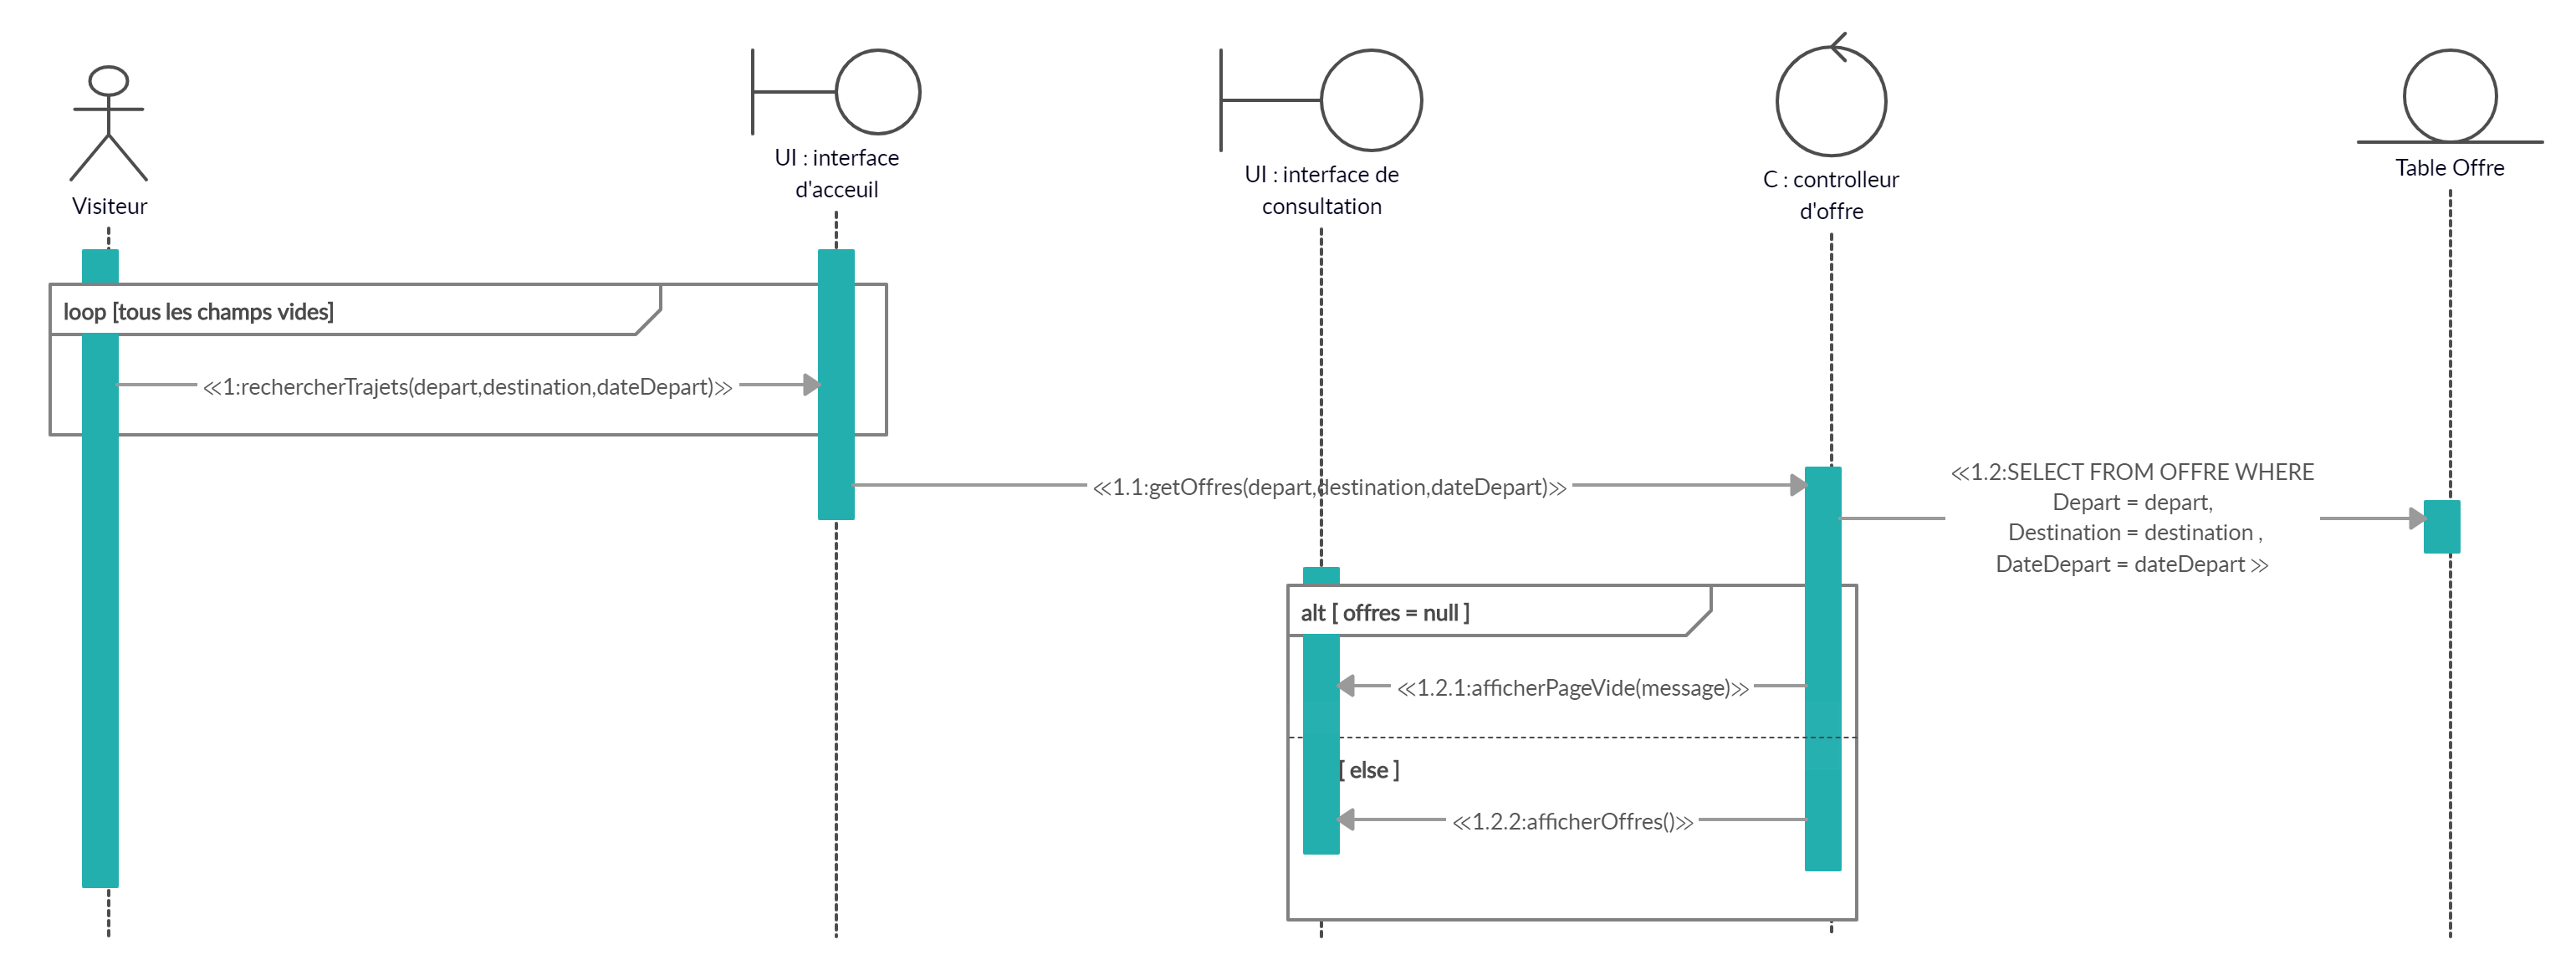
\includegraphics[angle=90,height=20cm]{Projet_JEE/SDconsulterOffres.jpg}
\end{center}
\caption[Consulter offres]{Consulter offres}
\end{figure}
\cleardoublepage
\item Diagramme de séquence créer compte :
\begin{figure}[!ht]
\begin{center}
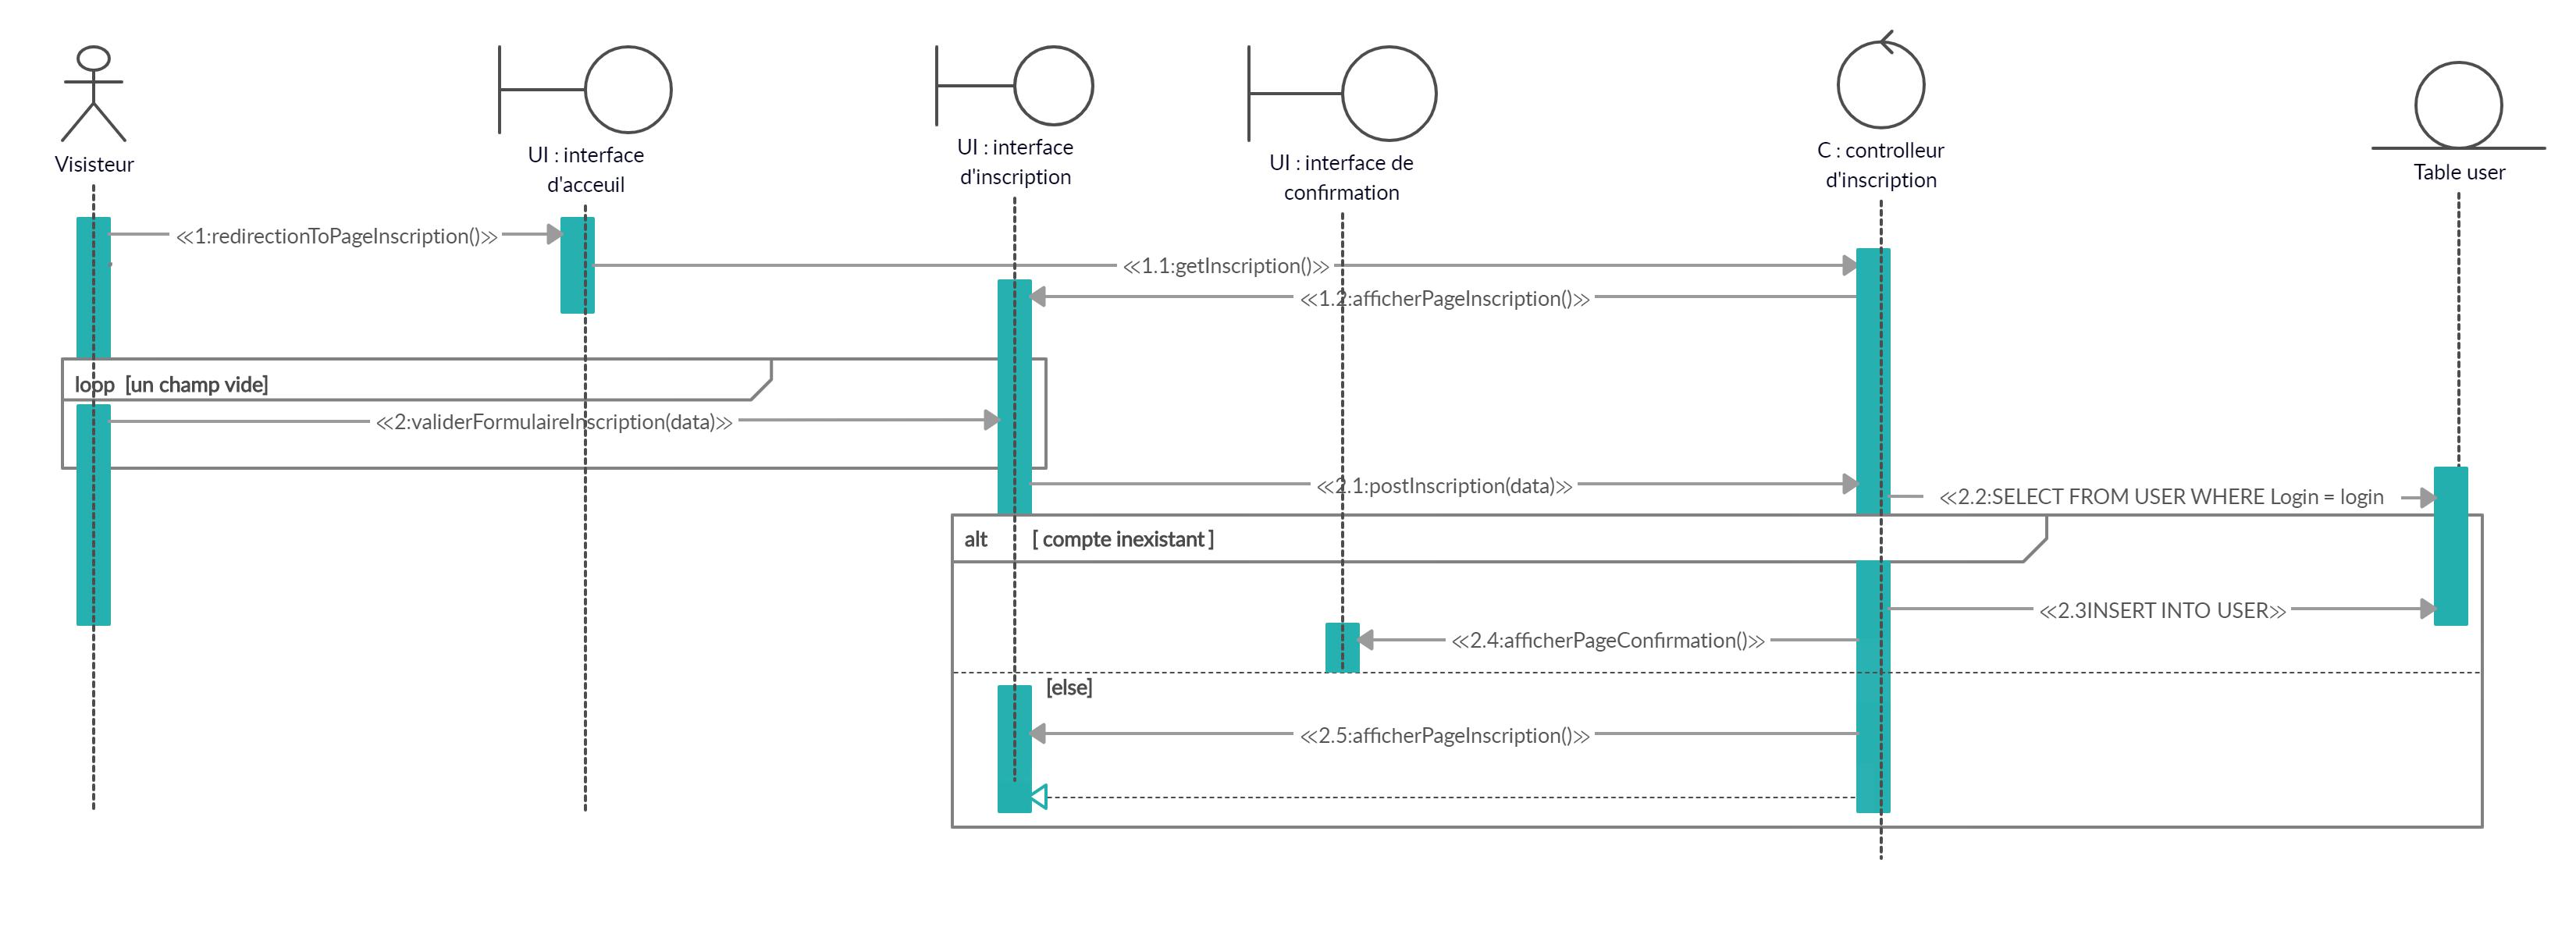
\includegraphics[angle=90,height=20cm]{Projet_JEE/SDcreerCompte.jpg}
\end{center}
\caption[Créer compte]{Créer compte}
\end{figure}
\cleardoublepage
\item Diagramme de séquence Choisir offre :
\begin{figure}[!ht]
\begin{center}
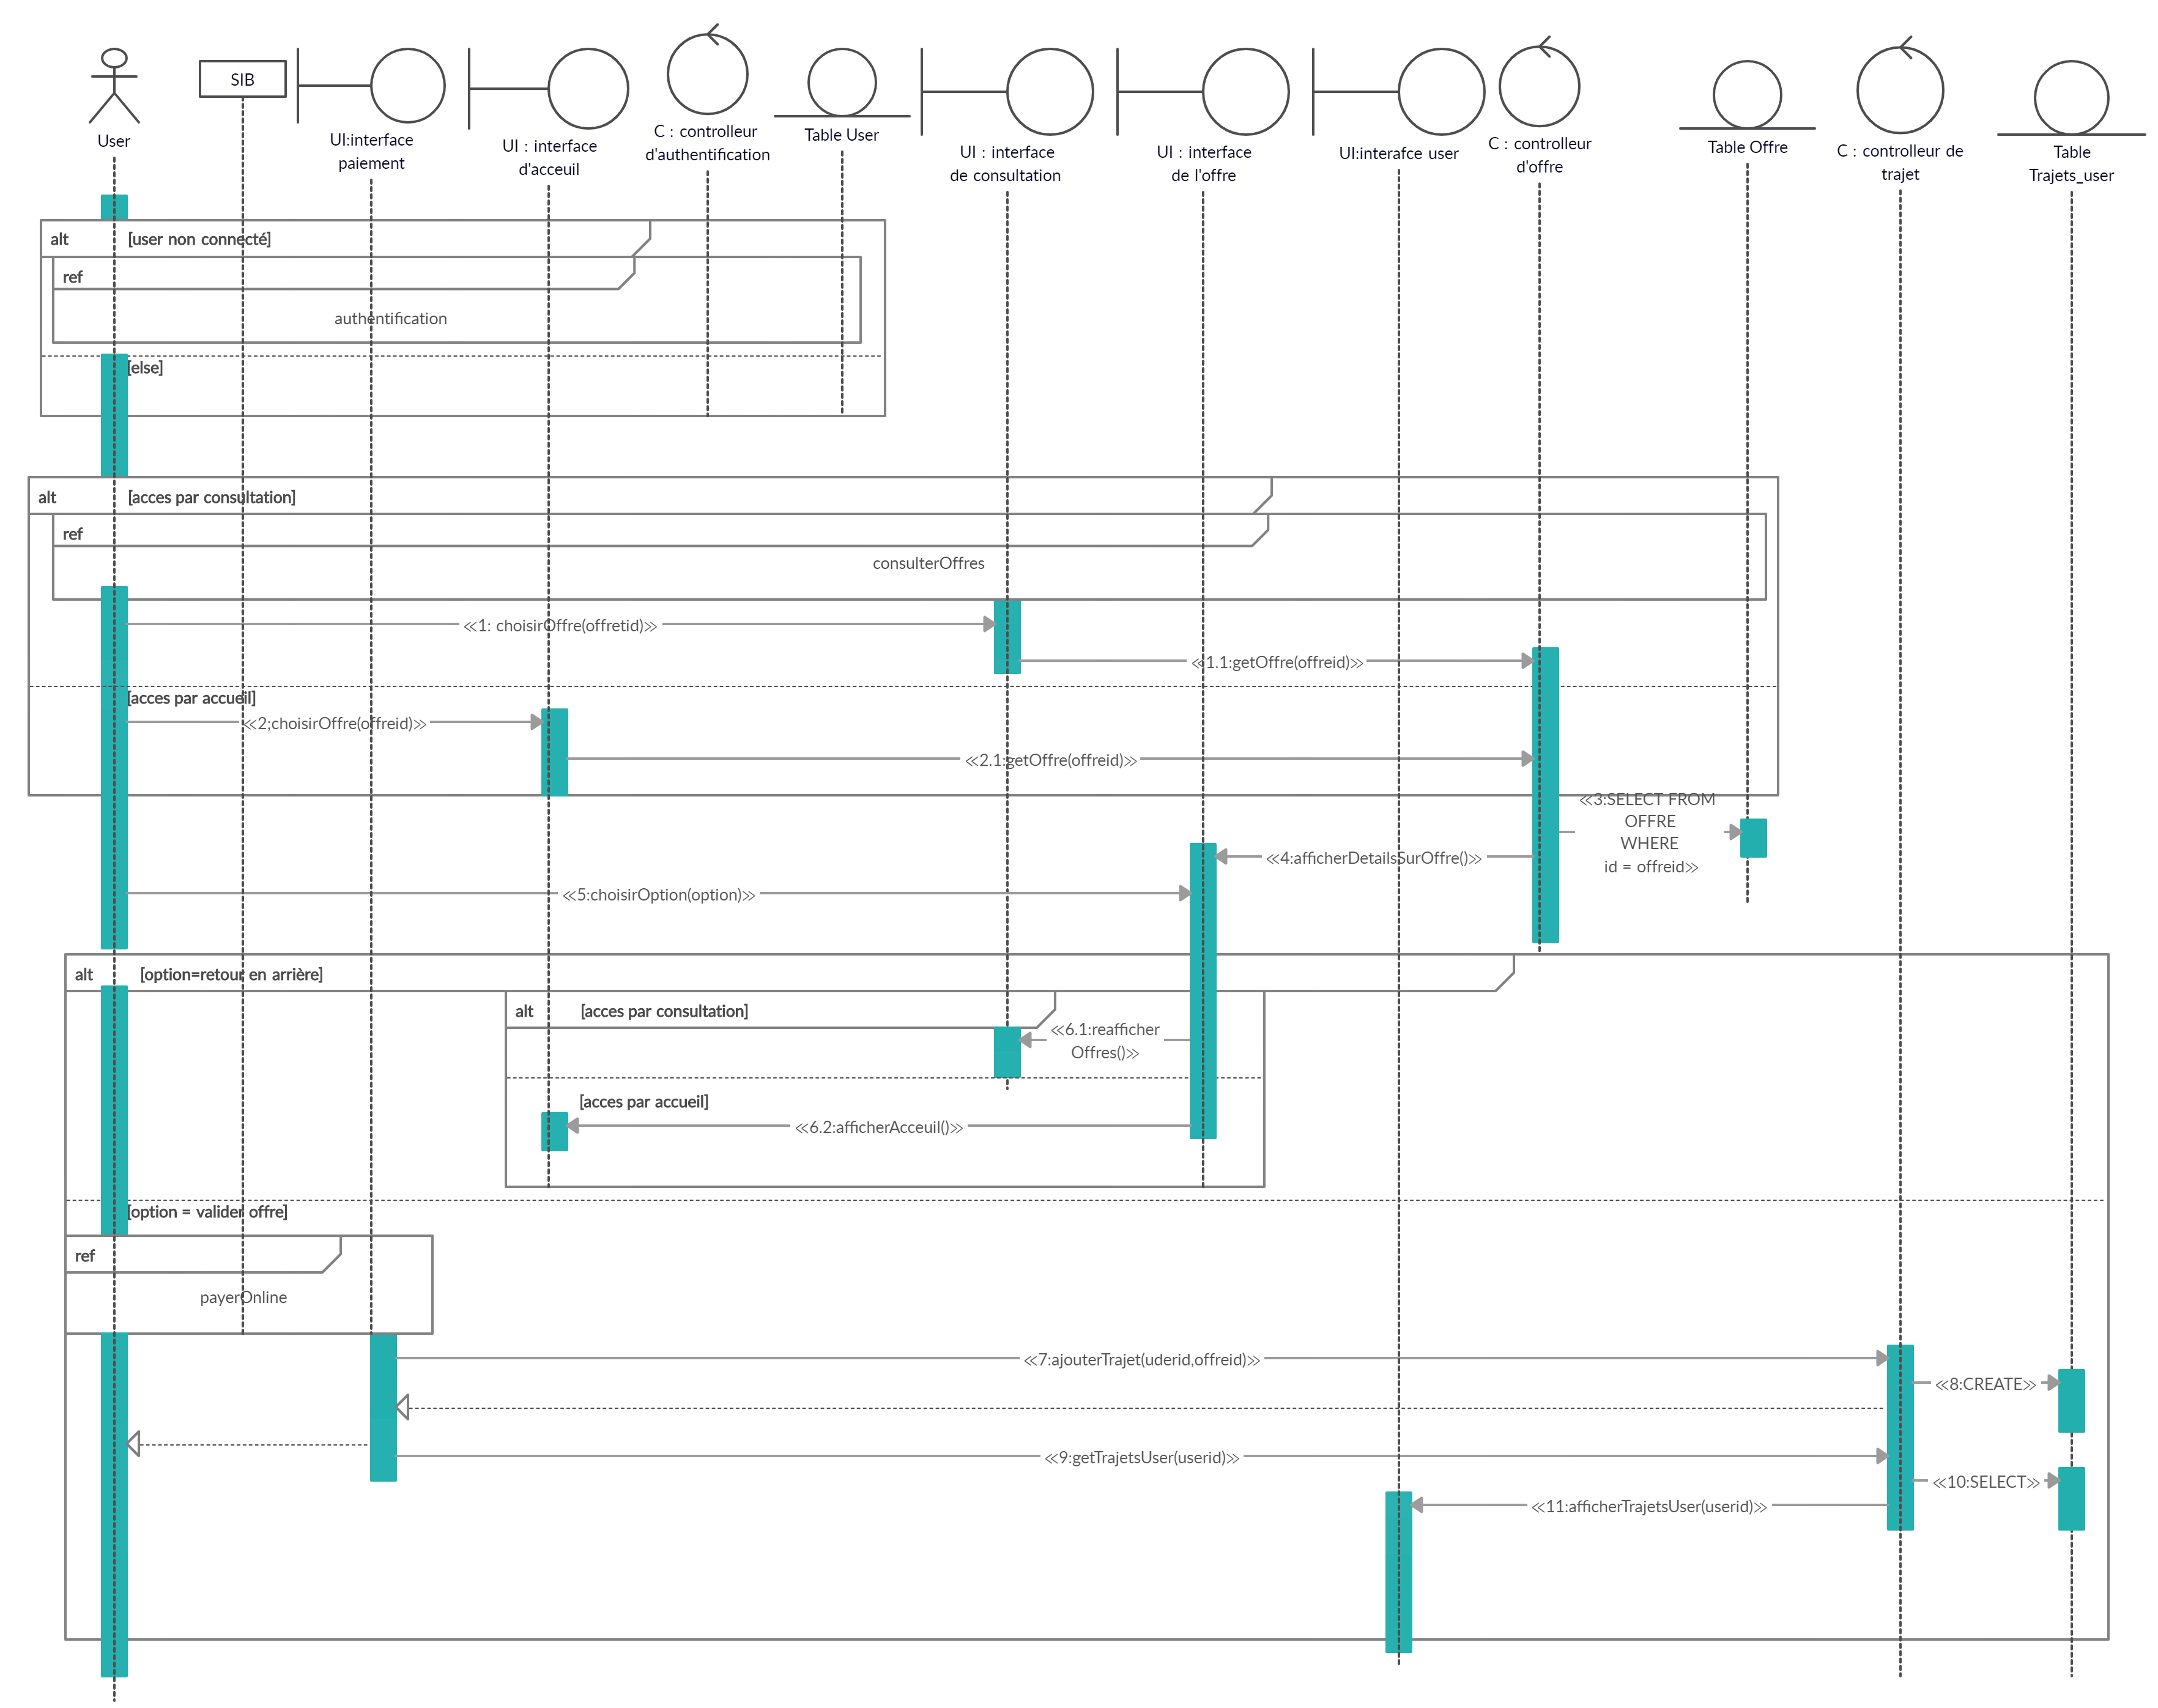
\includegraphics[angle=90,height=20cm]{Projet_JEE/SDchoisirOffre.jpg}
\end{center}
\caption[Choisir offres]{Choisir offres}
\end{figure}

\end{itemize}


\chapter{Maquettes de projet}
	
Une maquette est une représentation partielle ou complète d'un Système ou d'un objet (existant ou en projet) afin d'en tester et valider certains aspects et/ou le comportement (maquette fonctionnelle), ou simplement à des fins ludiques (maquette de jeu) ou informatives (présentation pédagogique ou commerciale d'une réalisation ou d'un projet).
Dans ce qui suit nous allez présenter les maquettes principales de notre site web .


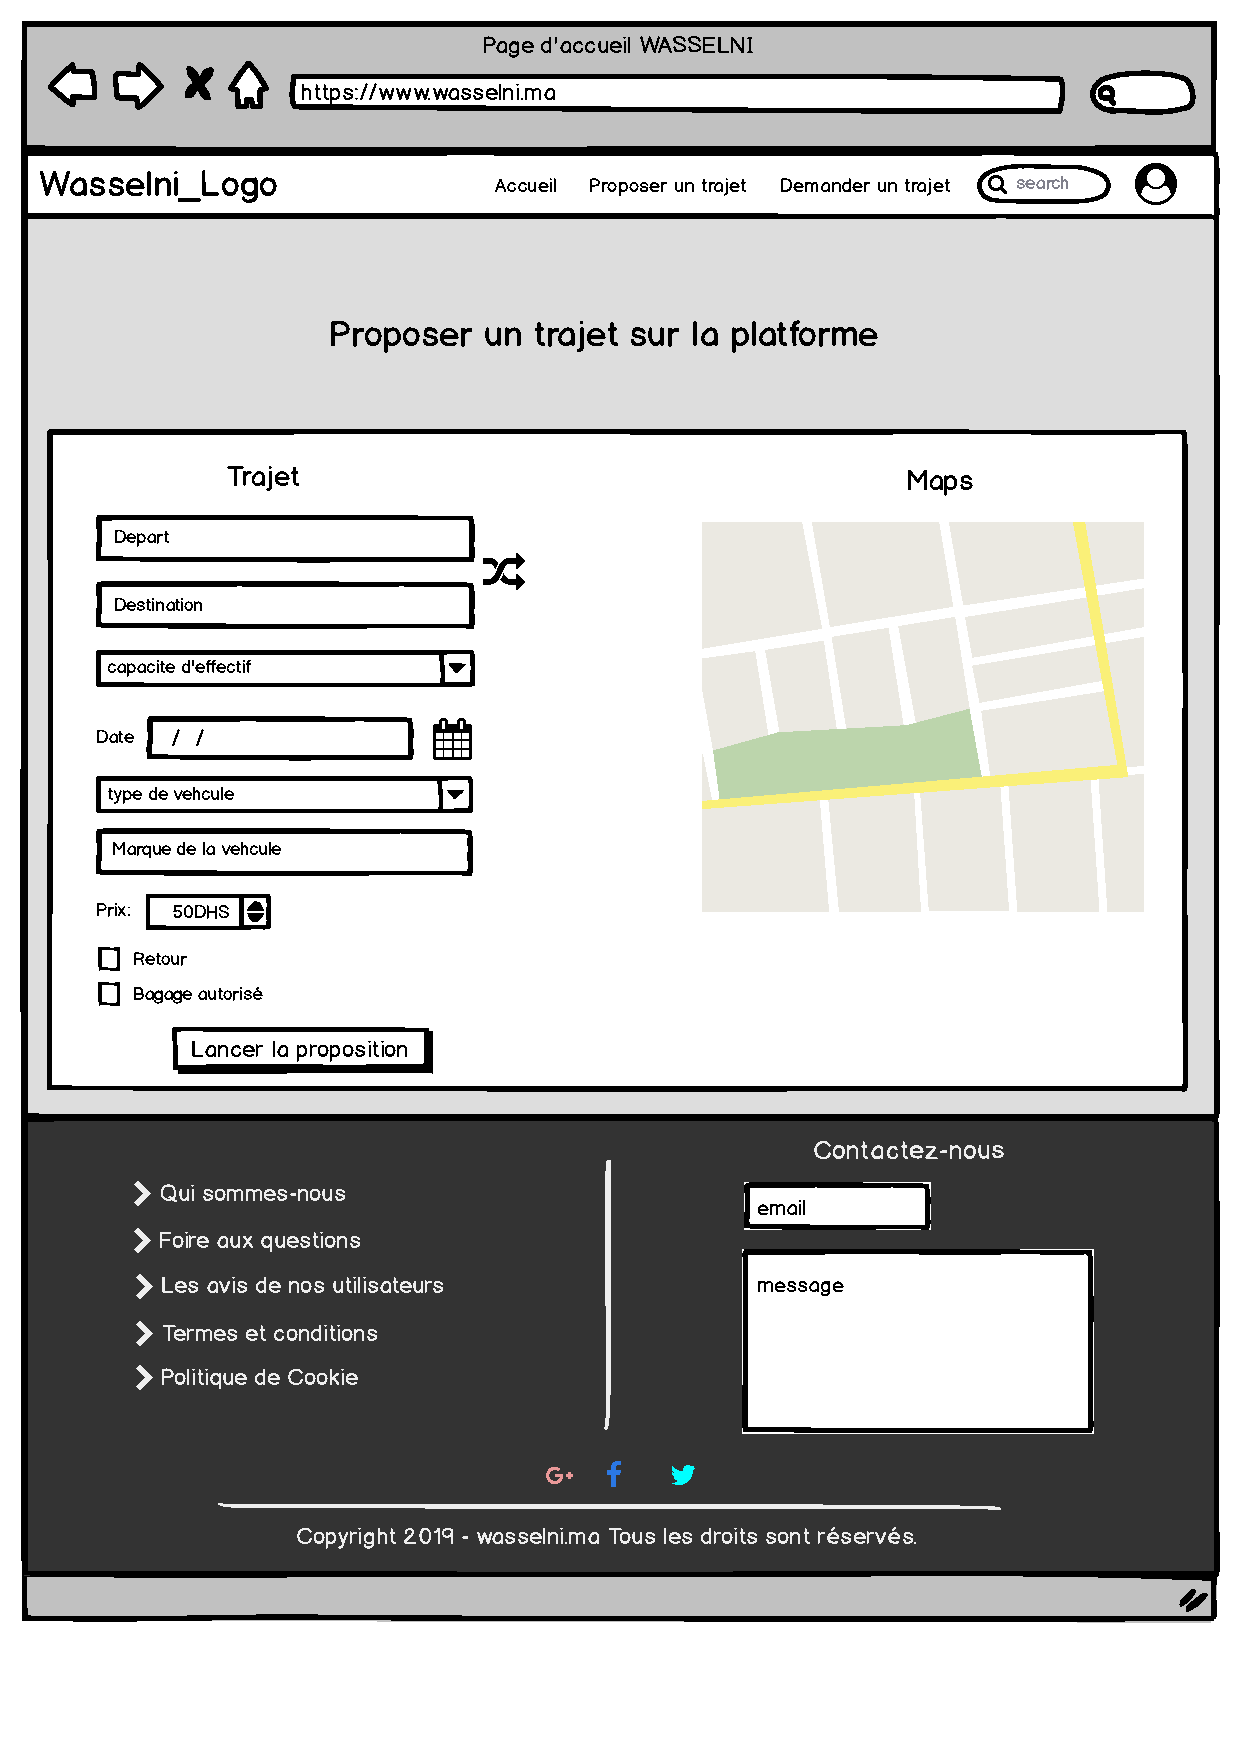
\includepdf[pages=-]{Projet_JEE/Maquette/proposer.pdf}

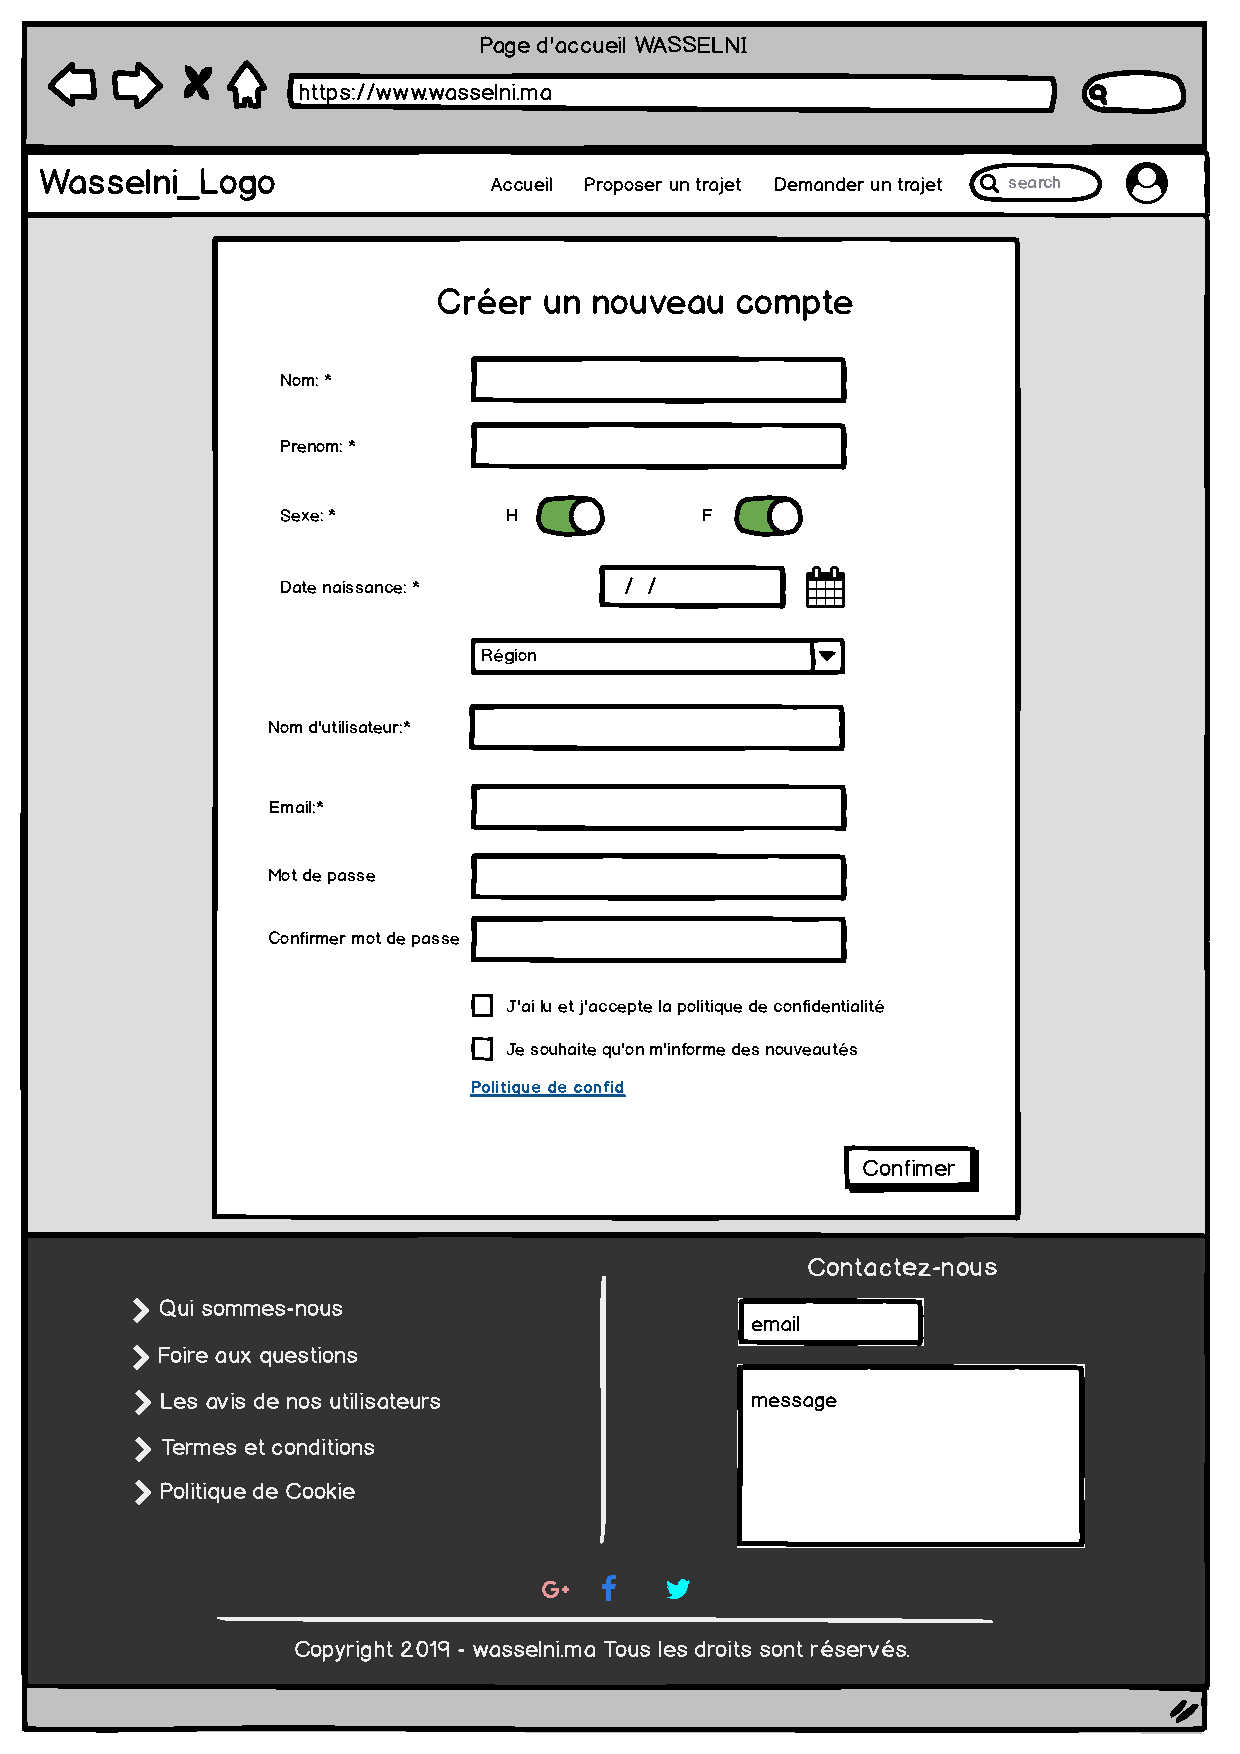
\includepdf[pages=-]{Projet_JEE/Maquette/inscription.pdf} 

 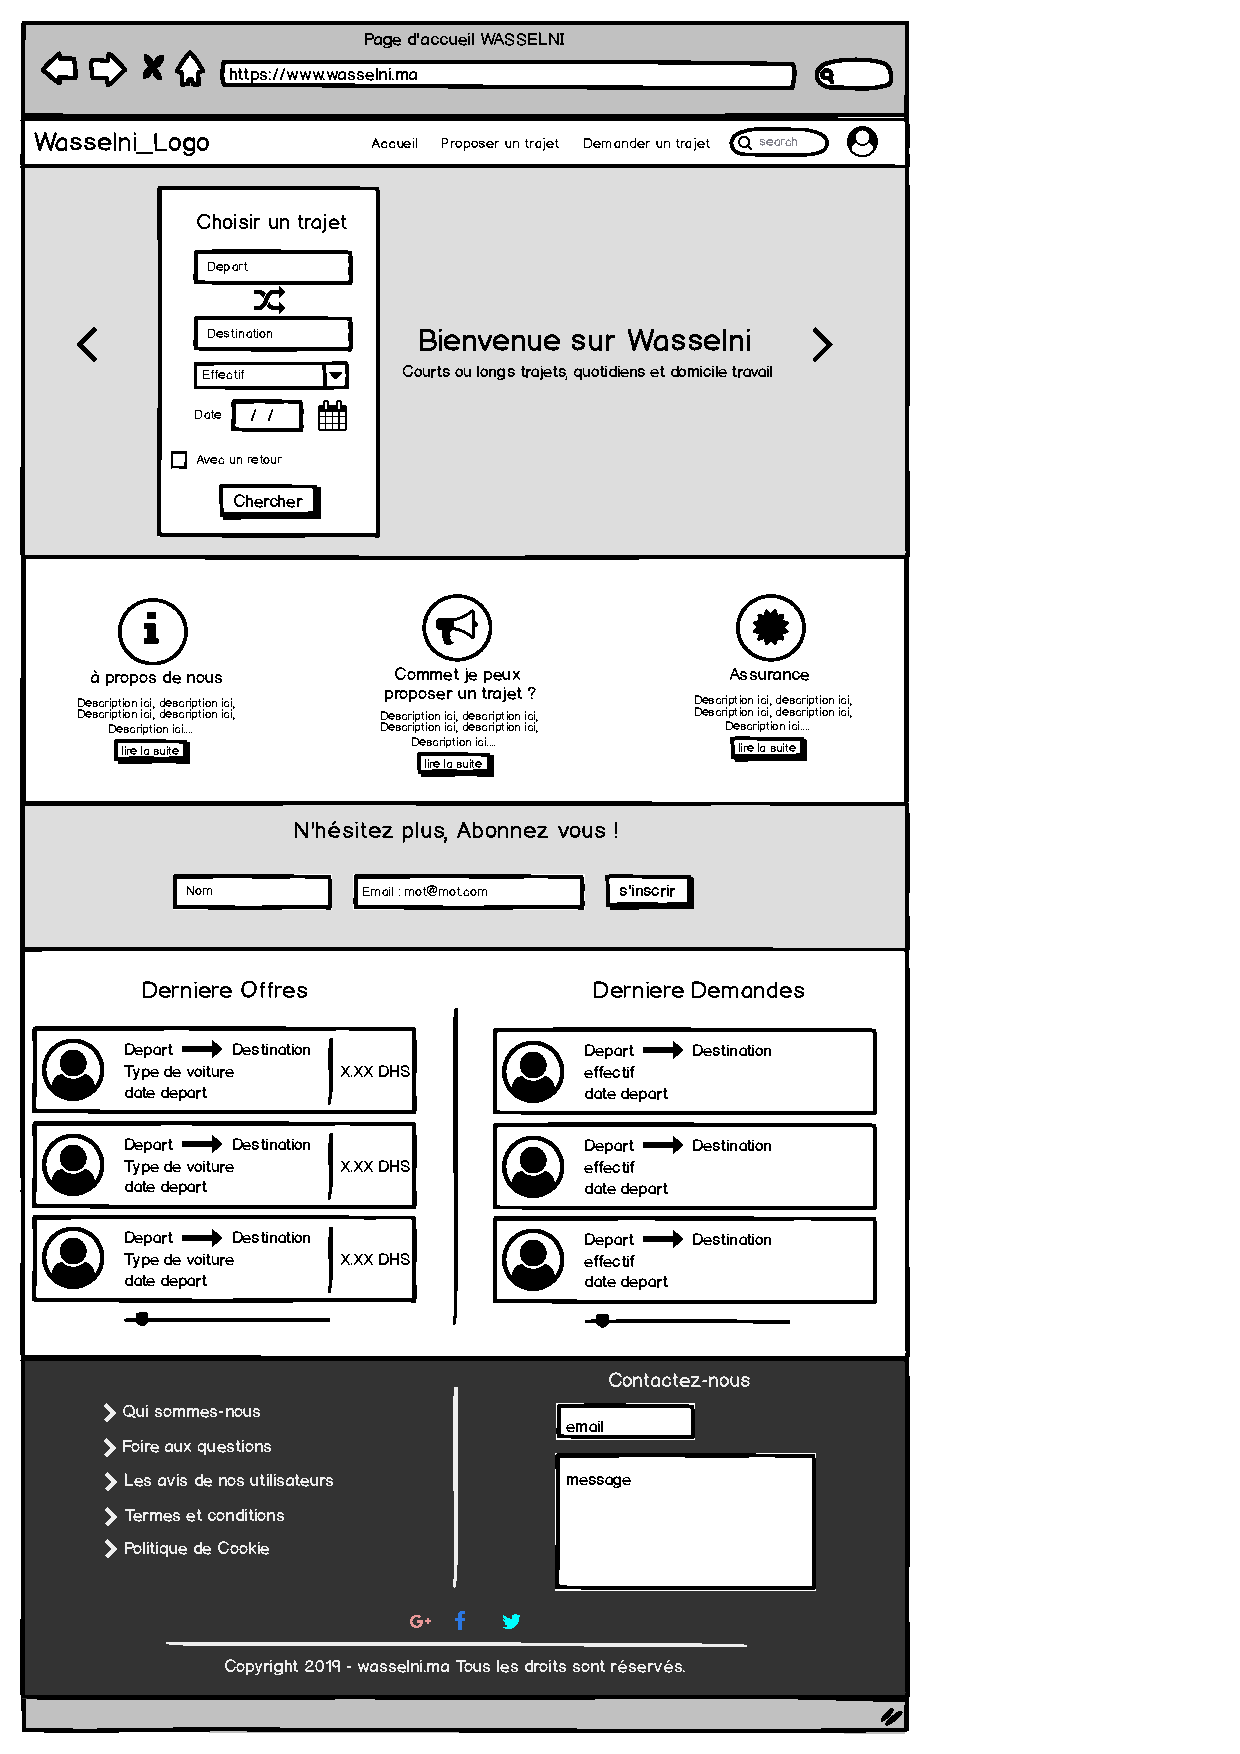
\includepdf[pages=-]{Projet_JEE/Maquette/home.pdf}

 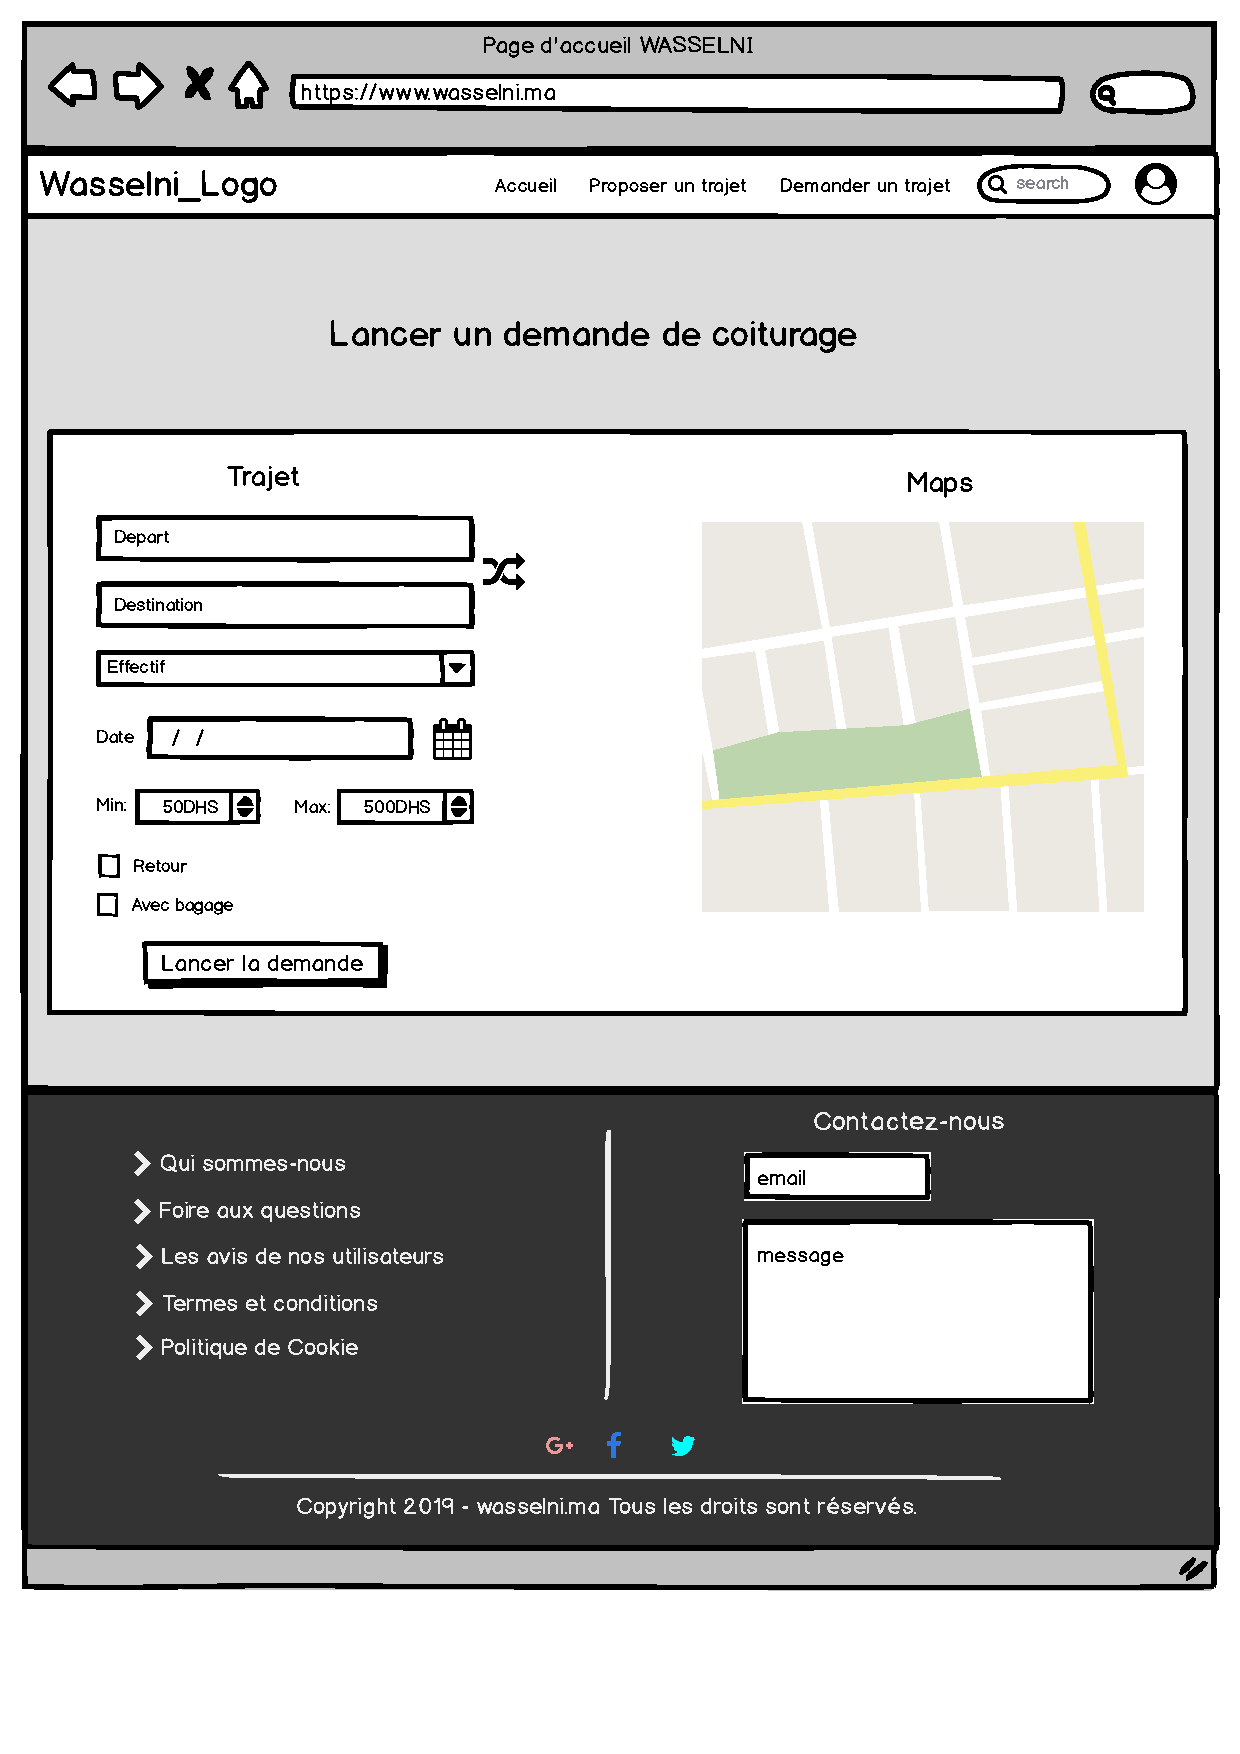
\includepdf[pages=-]{Projet_JEE/Maquette/demande.pdf}

 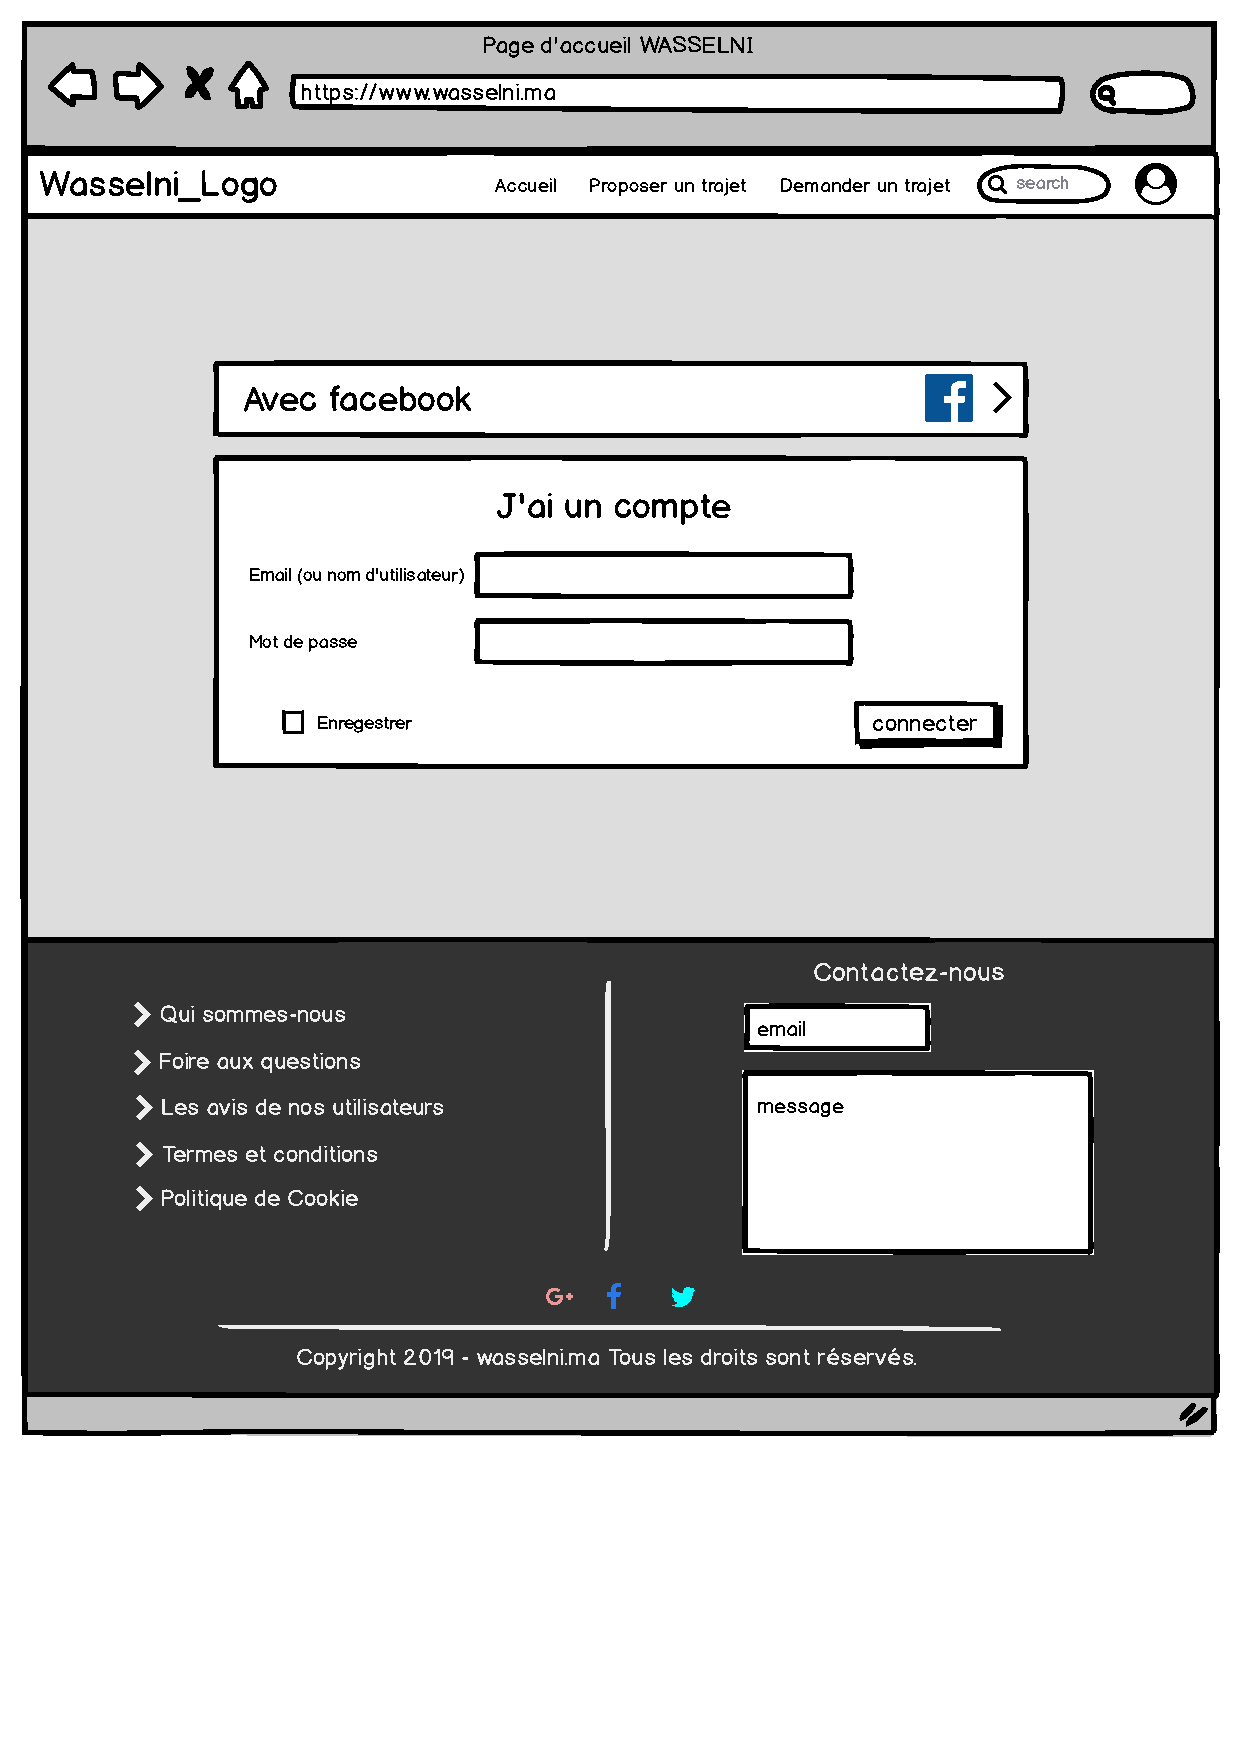
\includepdf[pages=-]{Projet_JEE/Maquette/authentification.pdf}



\chapter{Réalisation}
\section{les outils et les technologies}

\subsection{Pattern MVC}
Le pattern d'architecture logicielle MVC (\textbf{M}odèle-\textbf{V}ue-\textbf{C}ontrôleur) est un modèle destiné à répondre aux besoins des applications interactives en séparant les problématiques liées aux différents composants au sein de leur architecture respective..
Ce paradigme regroupe les fonctions nécessaires en trois catégories :\\
\begin{itemize}
\item[•] Un modèle : modèle de données.
\item[•] Une vue : interface utilisateur.
\item[•] Un contrôleur : logique de contrôle.\vspace{0.1cm}\\
\end{itemize}

\begin{minipage}{\linewidth}
	\makebox[\linewidth]{
		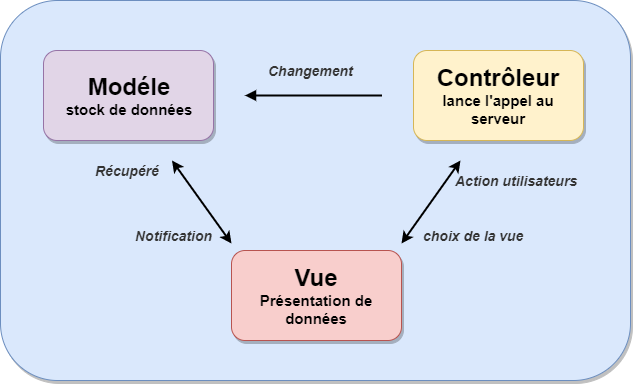
\includegraphics[keepaspectratio=true,scale=0.45]{image/mvc10}}
	\captionof{figure}{Pattern MVC.}\label{f3}%    
\end{minipage}\\
\cleardoublepage
Nous avons un premier découpage de l’application qui nous permet déjà de répondre à certaines de nos problématiques. En identifiant clairement les parties logiques, nous pouvons plus facilement maintenir notre application et la tester.\\
Voici les différents dossiers que nous avons utilisés pour appliquer le modèle MVC sur ce système:\\
\textbf{Package Controller:}\\
La partie Contrôleur gère la dynamique de l'application. Elle fait le lien entre l'utilisateur et le reste de l'application.\\
\begin{minipage}{\linewidth}
	\makebox[\linewidth]{
		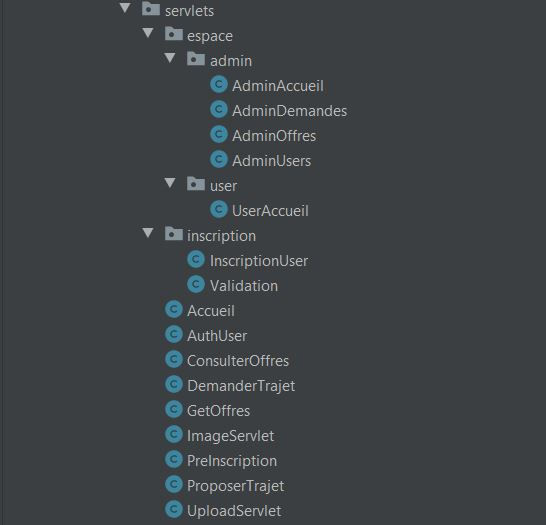
\includegraphics[keepaspectratio=true,scale=0.7]{image/bbb}}
	\captionof{figure}{Package Controller}\label{f11}%    
\end{minipage}
\textbf{Package Model:}\\
La partie Modèle d'une architecture MVC encapsule le logique métier  ainsi que l'accès aux données. Il peut s'agir d'un ensemble de fonctions (Modèle procédural) ou de classes (Modèle orienté objet).\\
\begin{minipage}{\linewidth}
	\makebox[\linewidth]{
		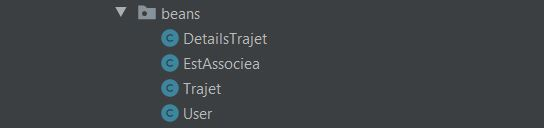
\includegraphics[keepaspectratio=true,scale=0.8]{image/ccc}}
	\captionof{figure}{Le sous package Data Access Object }\label{f9}%    
\end{minipage}\\
\textbf{Package View:}\\
La partie Vue s'occupe des interactions avec l'utilisateur : présentation, saisie et validation des données\\
\begin{minipage}{\linewidth}
	\makebox[\linewidth]{
		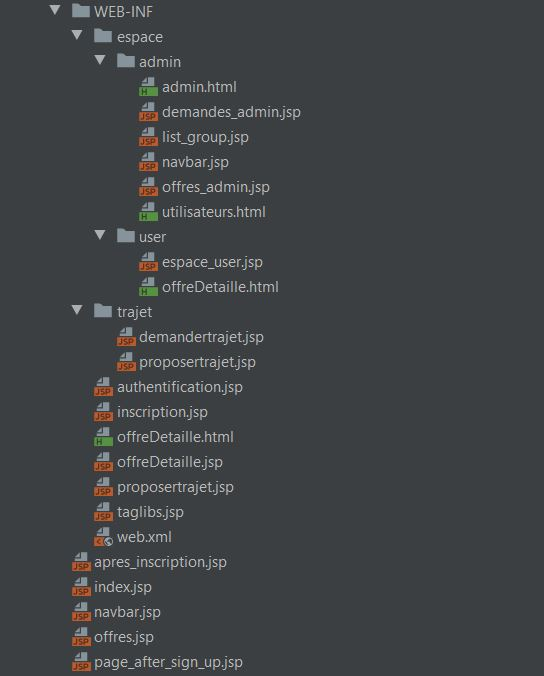
\includegraphics[keepaspectratio=true,scale=0.8]{image/ddd}}
	\captionof{figure}{Package View}\label{f10}%    
\end{minipage}\\


\subsection{Outils de développement }
\subsubsection{Langage de programmation}
\begin{minipage}{0.18\textwidth}
	\begin{minipage}{\linewidth}
	\makebox[\linewidth]{
		
\includegraphics[keepaspectratio=true,scale=0.4]{image/jee}}   
\end{minipage}
\end{minipage}
\hfill
\begin{minipage}{0.75\textwidth}
(Java Entreprise Edition) est la version entreprise de la plate-forme "Java" qui se compose de l'environnement "JSE" ainsi que de nombreuses API et composants destinés à une utilisation "côté serveur" au sein du système d'information de l'entreprise.\\
\textbf{\textit{Justification:}} JAVA est sécurisée, il a été conçu pour être exploité dans des environnements serveur et distribués. Dans ce cadre, la sécurité n’a pas été négligeable. C’est le langage le plus adopté par les développeurs grâce à sa fiabilité et sa performance élevé. \\
\end{minipage}\\
\subsubsection{Maven}
\begin{minipage}{0.2\textwidth}
	\begin{minipage}{\linewidth}
		\makebox[\linewidth]{
			
\includegraphics[keepaspectratio=true,scale=0.055]{image/maven}}   
	\end{minipage}
\end{minipage}
\hfill
\begin{minipage}{0.75\textwidth}
Apache Maven est un outil de gestion et d'automatisation de production des projets logiciels Java en général et Java EE en particulier. Il est utilisé pour automatiser l'intégration continue lors d'un développement de logiciel. Maven est géré par l'organisation Apache Software Foundation. L'outil était précédemment une branche de l'organisation Jakarta Project.\\
\end{minipage}\\
\subsubsection{Environnement de  développement}
\begin{minipage}{0.2\textwidth}
	\begin{minipage}{\linewidth}
		\makebox[\linewidth]{
			
\includegraphics[keepaspectratio=true,scale=0.04]{image/intellij}}   
	\end{minipage}
\end{minipage}
\hfill
\begin{minipage}{0.75\textwidth}
	IntelliJ IDEA également appelé « IntelliJ », « IDEA » ou « IDJ » est un environnement de développement intégré de technologie Java destiné au développement de logiciels informatiques. Il est développé par \textit{JetBrains} .\\
	\textbf{\textit{Justification:}} Un démarrage rapide et une prise en main progressive,. Un scope fonctionnel complet et une productivité accrue.\\
\end{minipage}\\
\subsubsection{Gestion de version \& collaboration:}
\begin{minipage}{0.2\textwidth}
	\begin{minipage}{\linewidth}
		\makebox[\linewidth]{
			
\includegraphics[keepaspectratio=true,scale=0.12]{image/git}}   
	\end{minipage}
\end{minipage}
\hfill
\begin{minipage}{0.75\textwidth}
	Git est un logiciel de gestion de versions décentralisé. C'est un logiciel libre créé par Linus Torvald, auteur du noyau Linux, et distribué selon les termes de la licence publique générale GNU version 2. En 2016, il s’agit du logiciel de gestion de versions le plus populaire qui est utilisé par plus de douze millions de personnes.\\
\end{minipage}\\

\begin{minipage}{0.2\textwidth}
	\begin{minipage}{\linewidth}
		\makebox[\linewidth]{
			
\includegraphics[keepaspectratio=true,scale=0.04]{image/github}}   
	\end{minipage}
\end{minipage}
\hfill
\begin{minipage}{0.75\textwidth}
GitHub est un service web d'hébergement et de gestion de développement de logiciels, utilisant le logiciel de gestion de versions Git. Ce site est développé en Ruby on Rails et Erlang par Chris Wanstrath, PJ Hyett et Tom Preston-Werner. GitHub propose des comptes professionnels payants, ainsi que des comptes gratuits pour les projets de logiciels libres. Le site assure également un contrôle d'accès et des fonctionnalités destinées à la collaboration comme le suivi des bugs, les demandes de fonctionnalités, la gestion de tâches et un wiki pour chaque projet.\\
\end{minipage}\\

\subsubsection{Design \& Multimédia:}
\begin{minipage}{0.2\textwidth}
	\begin{minipage}{\linewidth}
		\makebox[\linewidth]{
			
\includegraphics[keepaspectratio=true,scale=0.3]{image/html}}   
	\end{minipage}
\end{minipage}
\hfill
\begin{minipage}{0.75\textwidth}
	L'HyperText Markup Language, généralement abrégé HTML, est le langage de balisage conçu pour représenter les pages web. C'est un langage permettant d'écrire de l'hypertexte, d'où son nom.\\
\end{minipage}\\

\begin{minipage}{0.2\textwidth}
	\begin{minipage}{\linewidth}
		\makebox[\linewidth]{
			
\includegraphics[keepaspectratio=true,scale=0.04]{image/css}}   
	\end{minipage}
\end{minipage}
\hfill
\begin{minipage}{0.75\textwidth}
	Les feuilles de style en cascade, généralement appelées CSS de l'anglais Cascading Style Sheets, forment un langage informatique qui décrit la présentation des documents HTML et XML. Les standards définissant CSS sont publiés par le World Wide Web Consortium.\\
\end{minipage}\\
\begin{minipage}{0.28\textwidth}
	\begin{minipage}{\linewidth}
		\makebox[\linewidth]{
			
\includegraphics[keepaspectratio=true,scale=0.31]{image/js}}   
	\end{minipage}
\end{minipage}
\hfill
\begin{minipage}{0.75\textwidth}
	JavaScript (qui est souvent abrégé en « JS ») est un langage de script léger, orienté objet, principalement connu comme le langage de script des pages web.\\
\end{minipage}\vspace{0.5cm}\\
\begin{minipage}{0.2\textwidth}
	\begin{minipage}{\linewidth}
		\makebox[\linewidth]{
			
\includegraphics[keepaspectratio=true,scale=0.18]{image/eee}}   
	\end{minipage}
\end{minipage}
\hfill
\begin{minipage}{0.75\textwidth}
	La JavaServer Pages Standard Tag Library est un composant de la plate-forme JEE de développement. Elle étend la spécification JSP en ajoutant une bibliothéque de balises pour les taches courantes, comme le travail sur des fichiers XML, l'exécution conditionnelle, les boucles et l'internationalisation.
\end{minipage}\vspace{0.5cm}\\
\subsubsection{Serveur d’application:}
\begin{minipage}{0.2\textwidth}
	\begin{minipage}{\linewidth}
		\makebox[\linewidth]{
			
\includegraphics[keepaspectratio=true,scale=0.31]{image/tomcat}}   
	\end{minipage}
\end{minipage}
\hfill
\begin{minipage}{0.75\textwidth}
	Tomcat est un conteneur web libre de servlets et JSP. Issu du projet Jakarta, c'est un des nombreux projets de l’Apache Software Foundation.\\
\end{minipage}\\
\section{Présentation de \textit{Wasselni}}
Cette partie dénombre la présentation des Scénarios applicatifs de l’application. Nous allons présenter dans ce qui suit, les imprimes-écran des principales interfaces réalisées dans notre site web.
\subsection{Page d'accueil}
C’est la page d’accueil qui s’affiche dès l’accès à notre site web, elle est constituer de trois parties principales :\\
$\bullet$ Un champ de recherche donnant aux visiteurs de notre plateforme le choix de sélection offres de covoiturage selon les lieu de départe et destination, la date, l'effectif, et le prix par passager.\\
$\bullet$ Un slider animé donnant un flash sur les derniers offres.\\
$\bullet$ Un slider animé donnant un flash sur les derniers demandes.\\ 
\begin{figure}[!ht]
\begin{center}
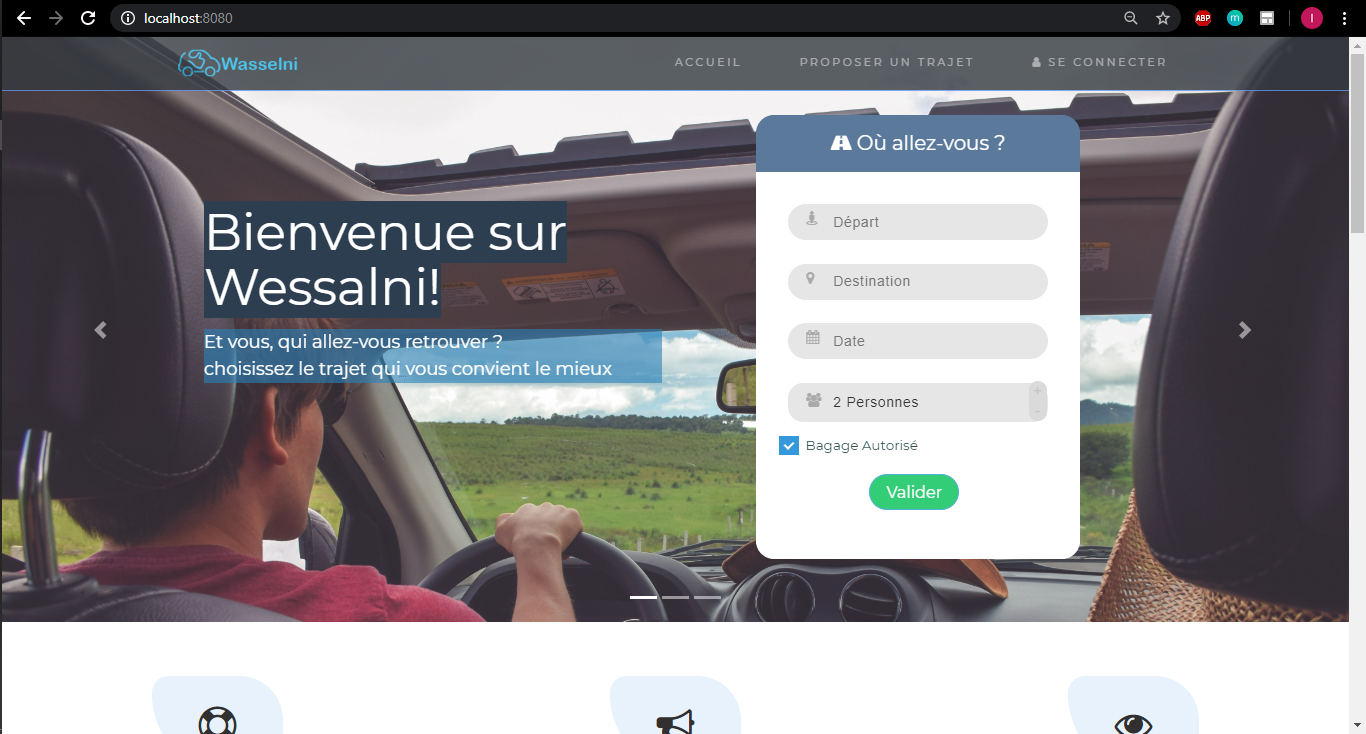
\includegraphics[height=9.5cm]{accueil1.png}
\end{center}
\caption[Page d'accueil]{Page d'accueil}
\end{figure}
\begin{figure}[!ht]
\begin{center}
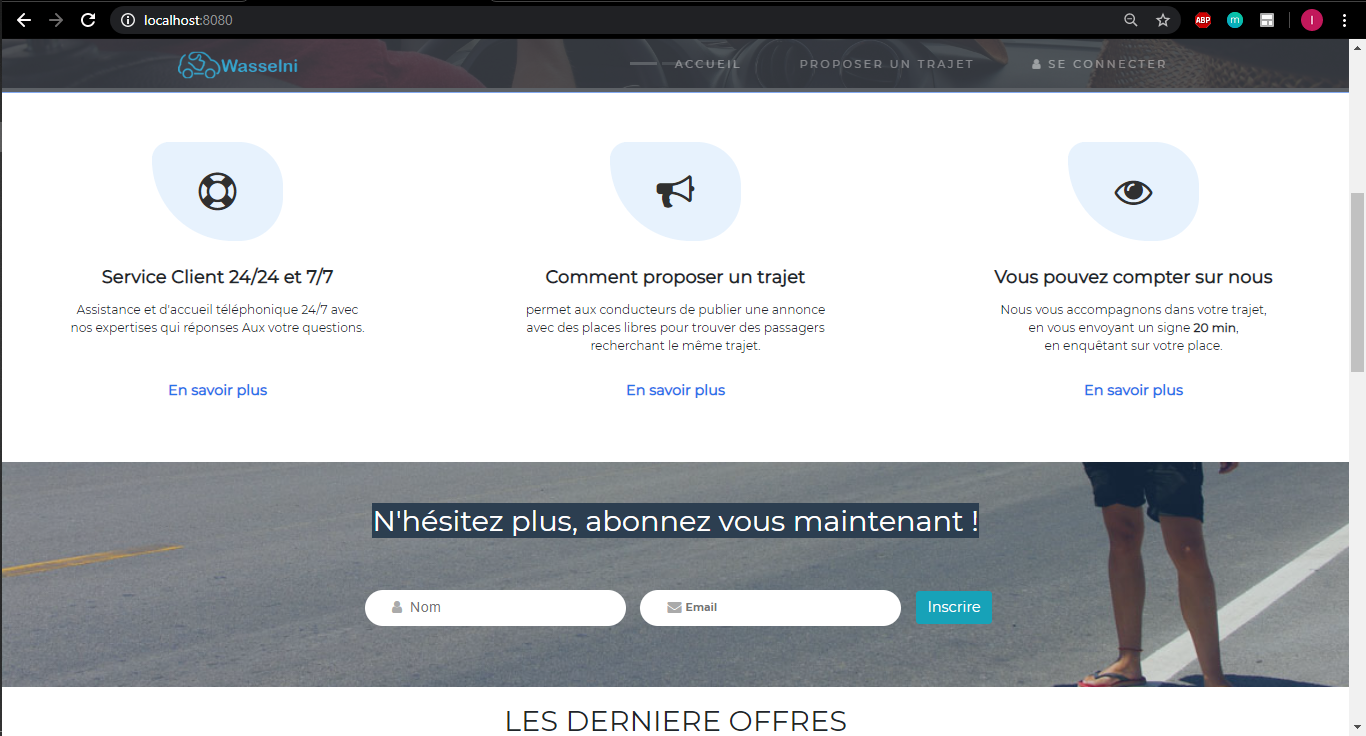
\includegraphics[height=9.5cm]{accueil2.png}
\end{center}
\caption[Page d'accueil]{Page d'accueil}
\end{figure}
\begin{figure}[!ht]
\begin{center}
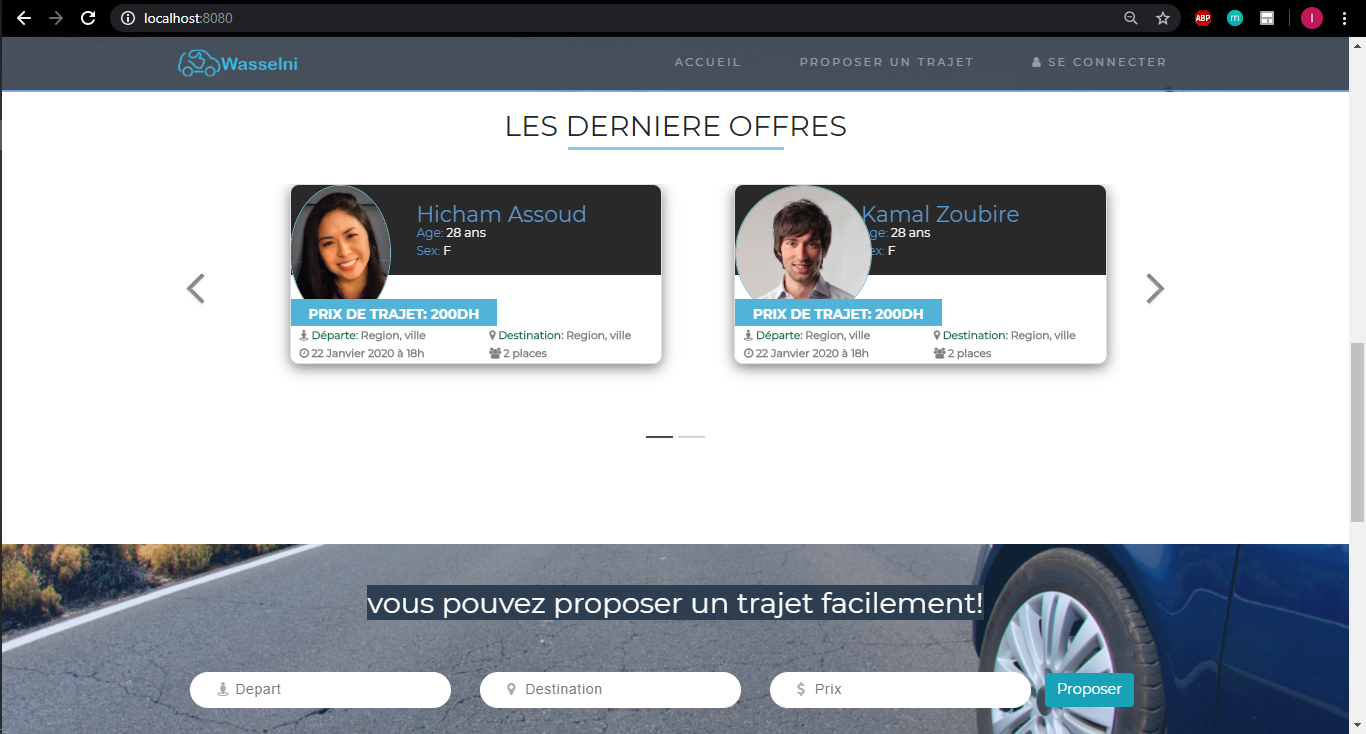
\includegraphics[height=9.5cm]{accueil3.png}
\end{center}
\caption[Page d'accueil]{Page d'accueil}
\end{figure}
\begin{figure}[!ht]
\begin{center}
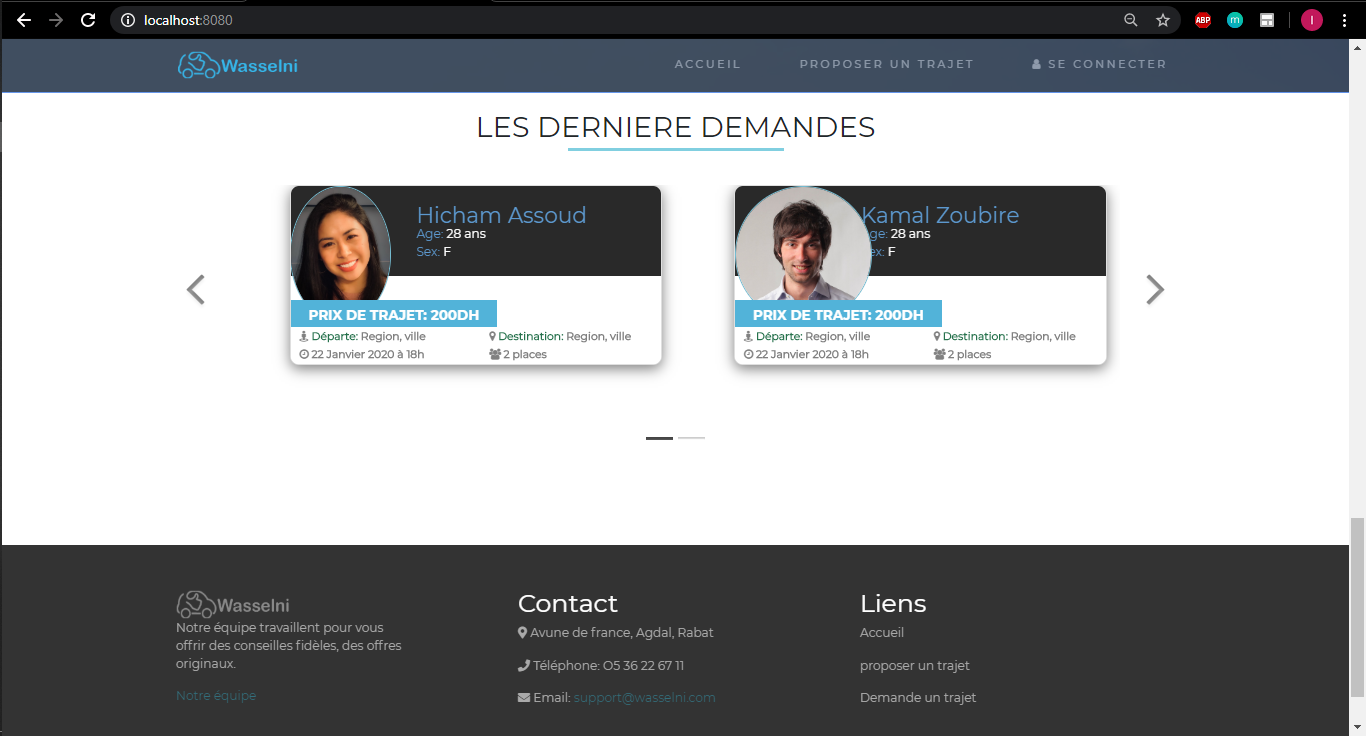
\includegraphics[height=9.5cm]{accueil4.png}
\end{center}
\caption[Page d'accueil]{Page d'accueil}
\end{figure}
\subsection{Page d'inscription}
Comme dans tout les plateforme en ligne, le visiteur ne peut profiter des activités qu’après la phase d’inscription, notre site web met à la disposition de ses visiteurs un formulaire d’inscription.\\ 
\begin{figure}[!ht]
\begin{center}
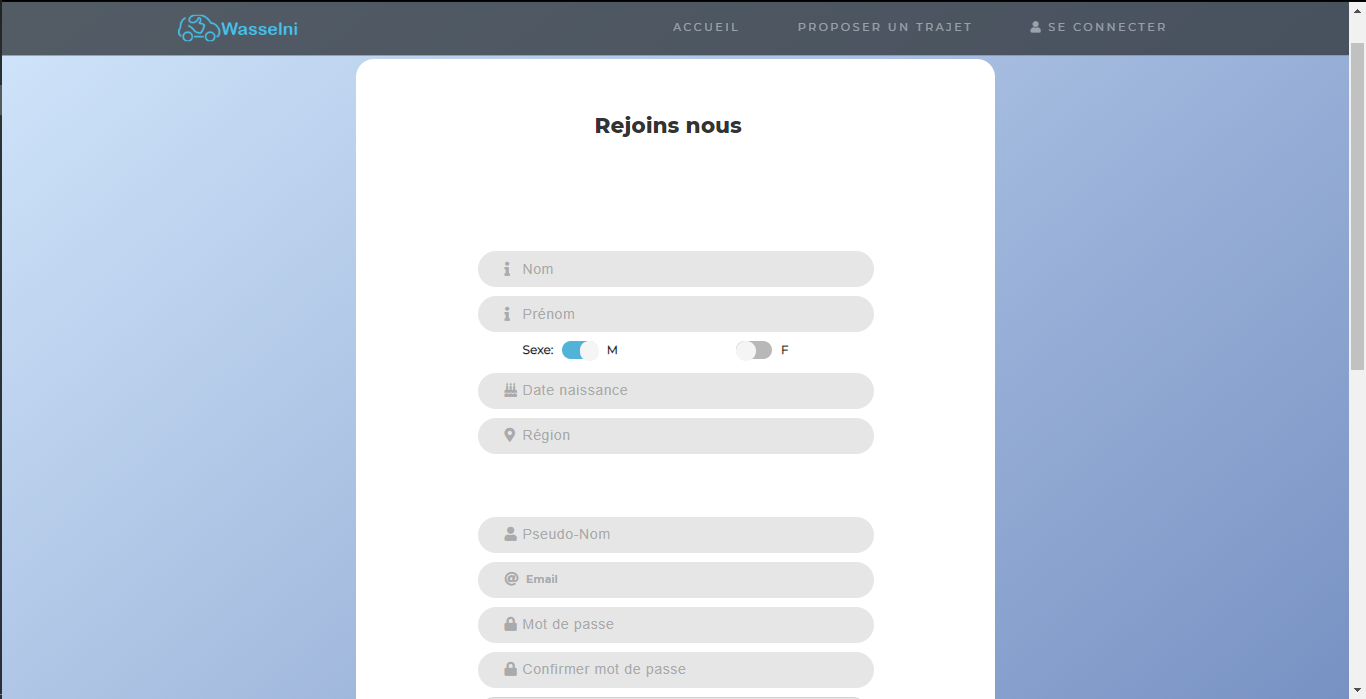
\includegraphics[height=9cm]{insc1.png}
\end{center}
\caption[Page d'inscription]{Page d'inscription}
\end{figure}
\begin{figure}[!ht]
\begin{center}
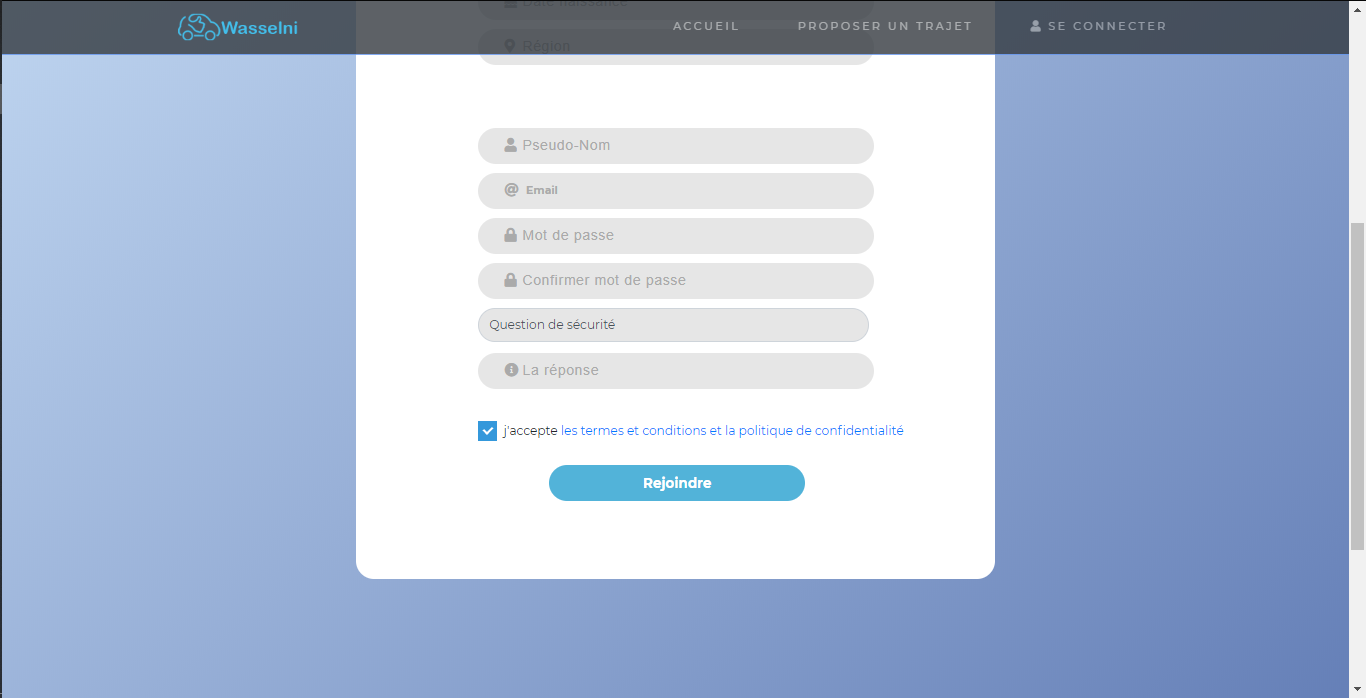
\includegraphics[height=9cm]{insc2.png}
\end{center}
\caption[Page d'inscription]{Page d'inscription}
\end{figure}

\subsection{Page d'authentification}
Après la phase d’inscription présentée dans la figure précédant l'utilisateur  doit s’authentifier pour bien profiter des privilèges qu’un visiteur normal ne possède pas comme par exemple pour proposer un offre ou bien un demande.\\ 
\begin{figure}[!ht]
\begin{center}
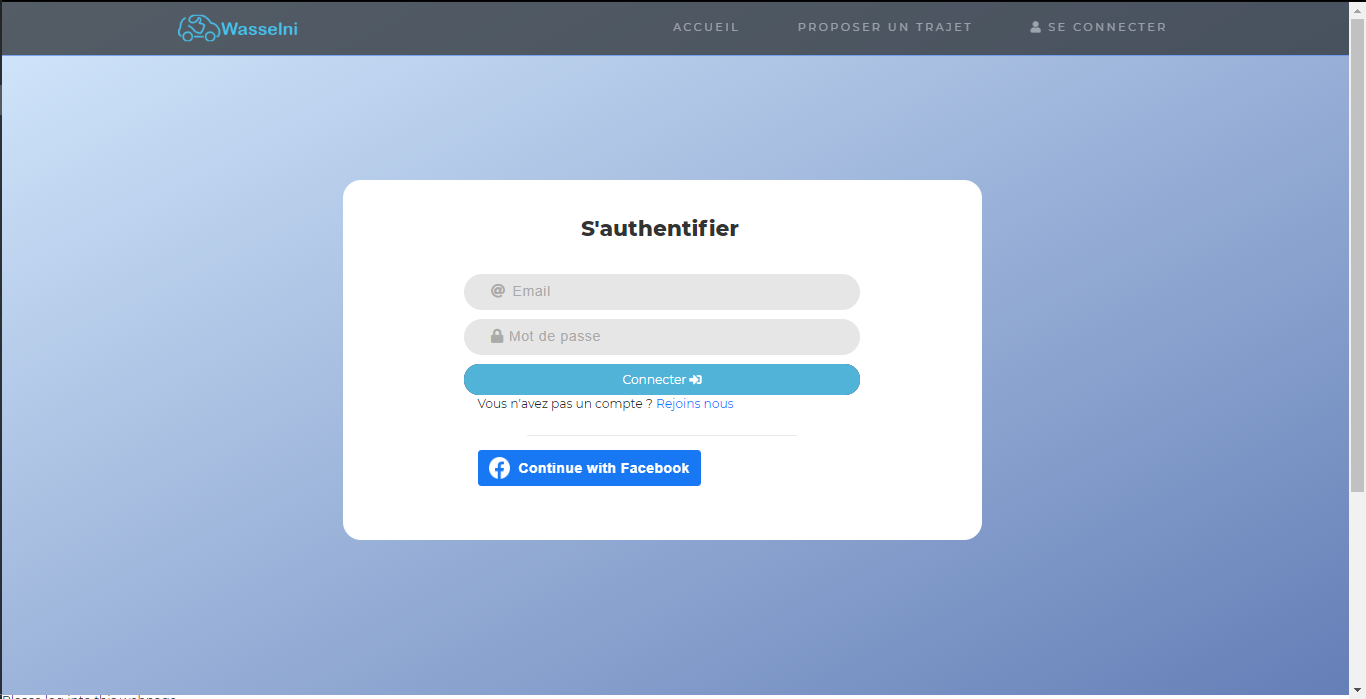
\includegraphics[height=9cm]{auth.png}
\end{center}
\caption[Page authentification]{Page authentification}
\end{figure}

\subsection{Liste des offres}
Liste des offres disponibles, le visiteur peut sélectionner les offres selon plusieurs critères (départ, destination, date, prix).\\ 
\begin{figure}[!ht]
\begin{center}
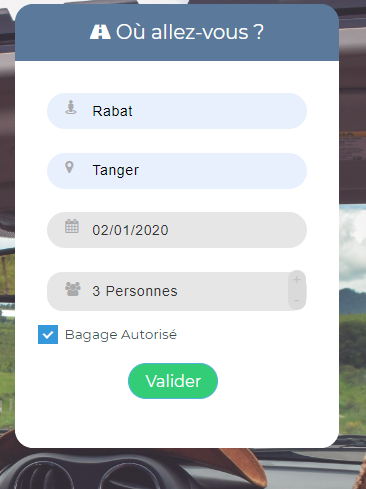
\includegraphics[height=9.5cm]{offre1.png}
\end{center}
\caption[Page offres]{Page offres}
\end{figure}

\subsection{Proposer trajet}
La page proposer trajet permettre au visiteur proposer un trajet en remplissant les informations nécessaire concernant le trajet.\\ 
\begin{figure}[!ht]
\begin{center}
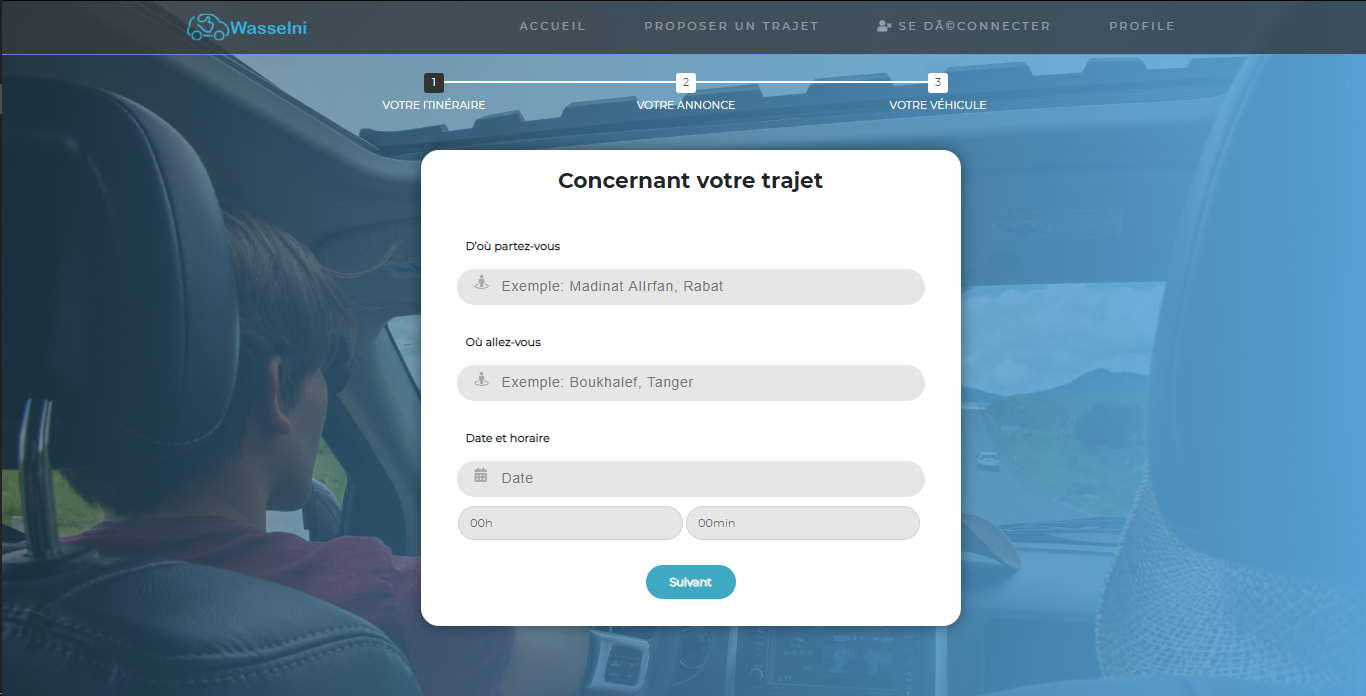
\includegraphics[height=9cm]{propo1.png}
\end{center}
\caption[Page proposer trajet]{Page proposer trajet}
\end{figure}
\begin{figure}[!ht]
\begin{center}
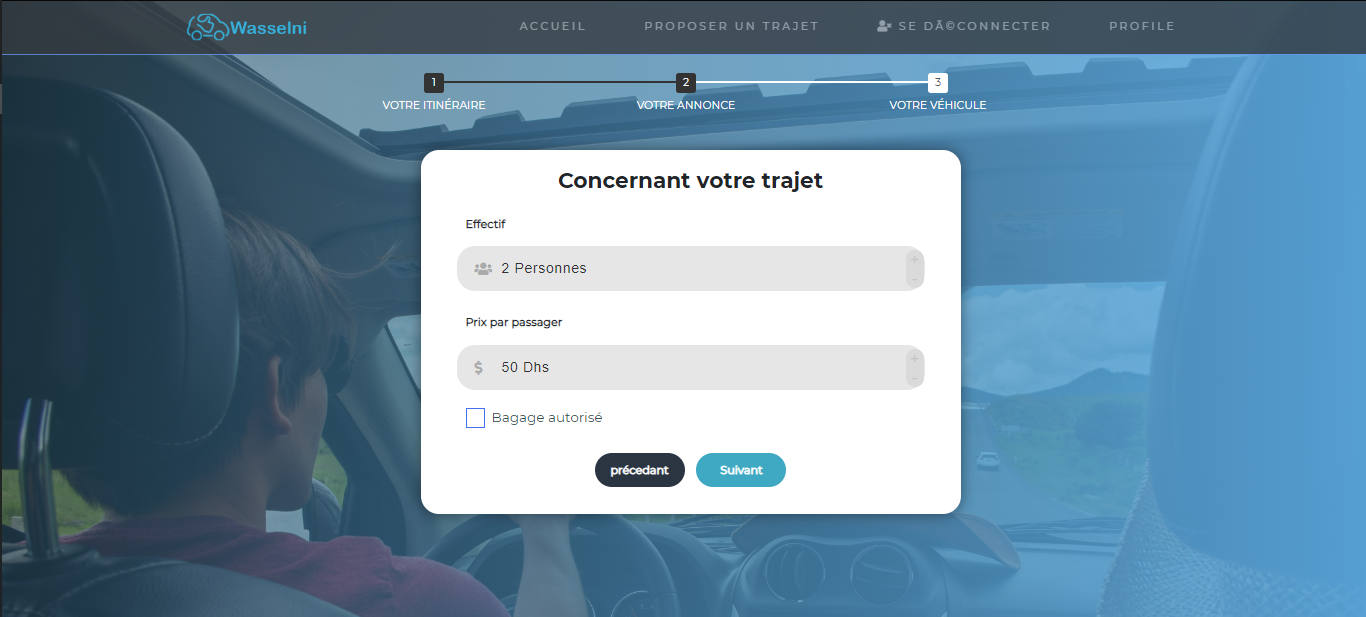
\includegraphics[height=8cm]{propo2.png}
\end{center}
\caption[Page proposer trajet]{Page proposer trajet}
\end{figure}
\begin{figure}[!ht]
\begin{center}
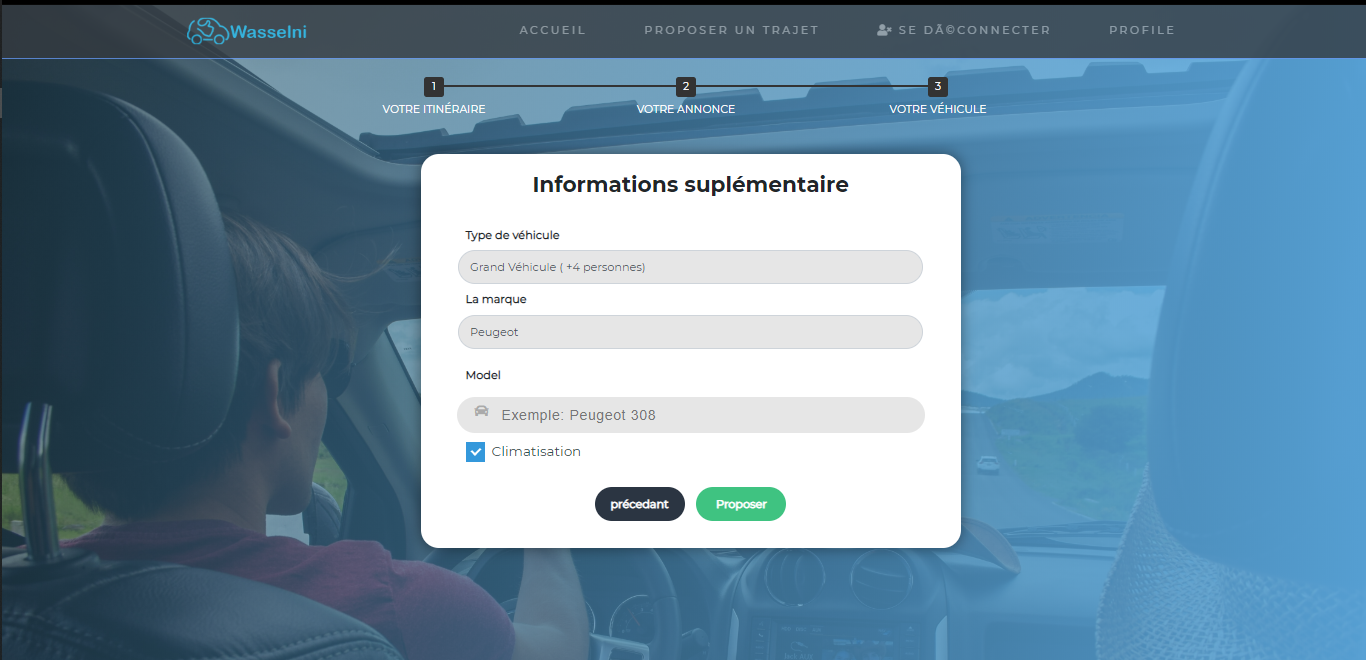
\includegraphics[height=8.5cm]{propo3.png}
\end{center}
\caption[Page proposer trajet]{Page proposer trajet}
\end{figure}

\subsection{Espace user}
Cette page représente des informations détailler d'un compte utilisateur, ainsi leur reviews sous forme des pourcentages, et bien sur un historique de leur offres/demandes\\ 
\begin{figure}[!ht]
\begin{center}
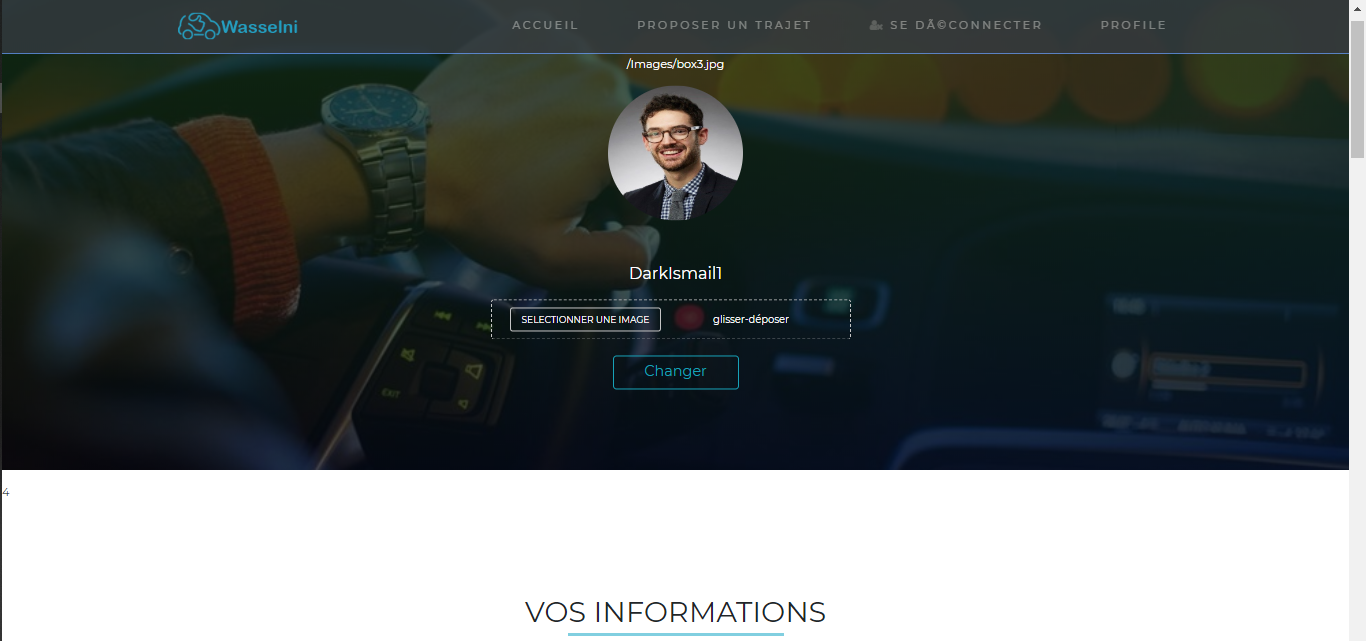
\includegraphics[height=8cm]{user1.png}
\end{center}
\caption[Espace user]{Espace user}
\end{figure}

\begin{figure}[!ht]
\begin{center}
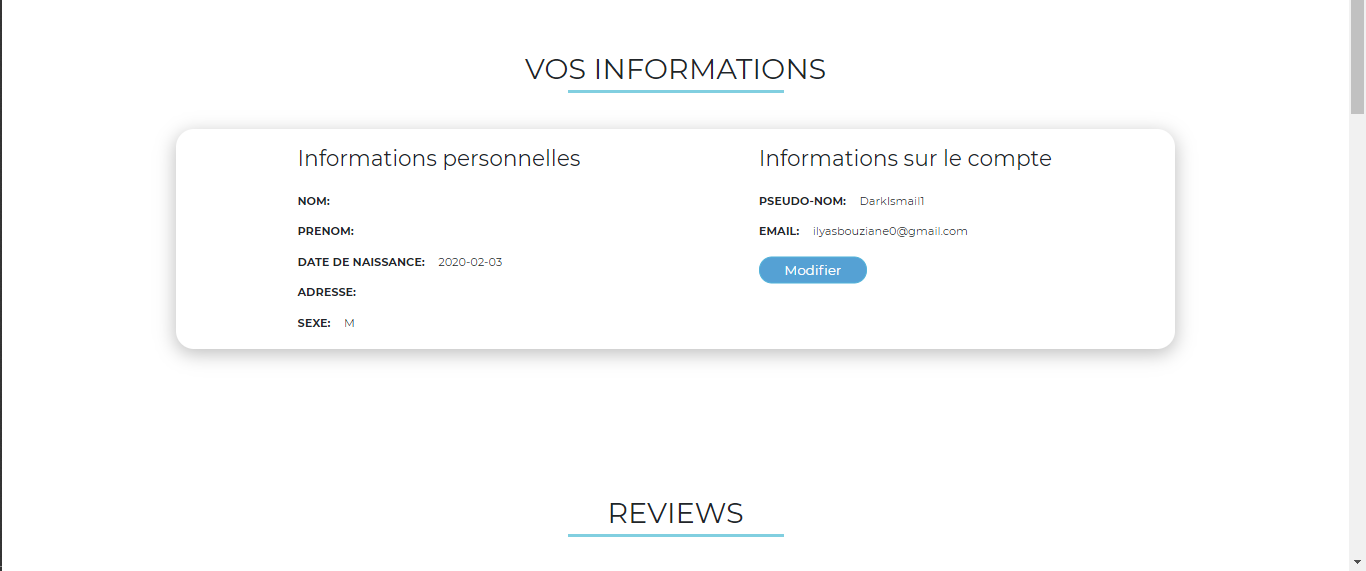
\includegraphics[height=8cm]{user2.png}
\end{center}
\caption[Espace user]{Espace user}
\end{figure}

\begin{figure}[!ht]
\begin{center}
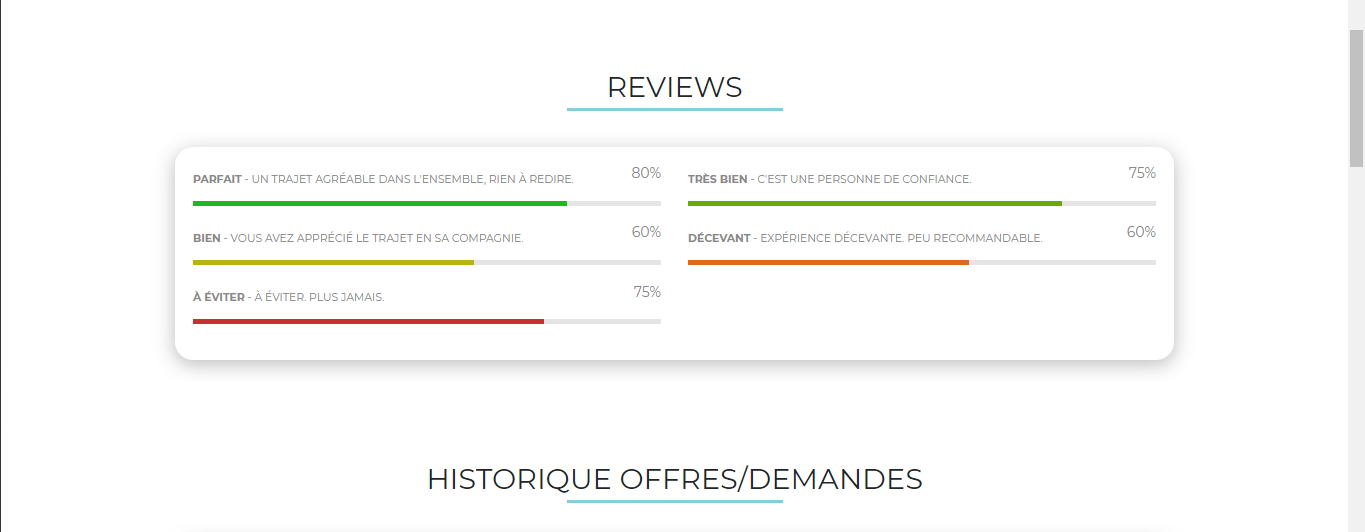
\includegraphics[height=8cm]{user3.png}
\end{center}
\caption[Espace user]{Espace user}
\end{figure}

\begin{figure}[!ht]
\begin{center}
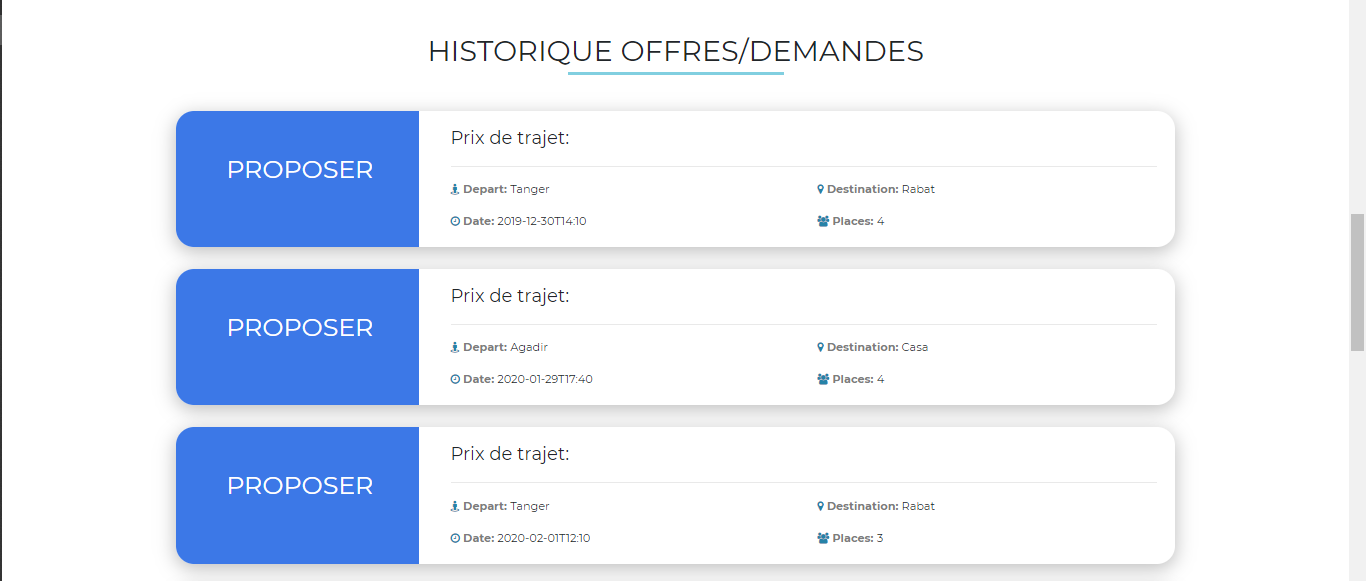
\includegraphics[height=8cm]{user4.png}
\end{center}
\caption[Espace user]{Espace user}
\end{figure}
\cleardoublepage

\subsection{Espace admin}
Une page permet de gérer le contenu et les fonctionnalités du site. Cette partie n'est pas visible par les internautes.
\begin{figure}[!ht]
\begin{center}
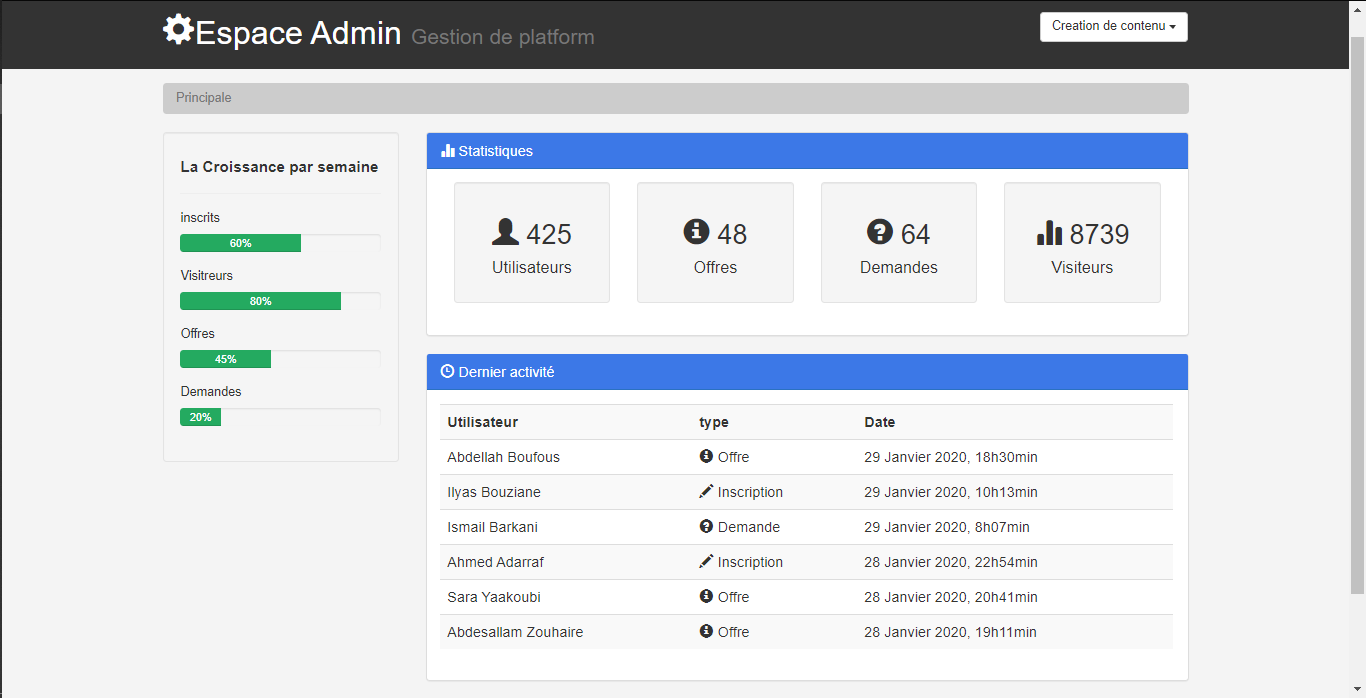
\includegraphics[height=8cm]{admin1.png}
\end{center}
\caption[Espace admin]{Espace admin}
\end{figure}
\begin{figure}[!ht]
\begin{center}
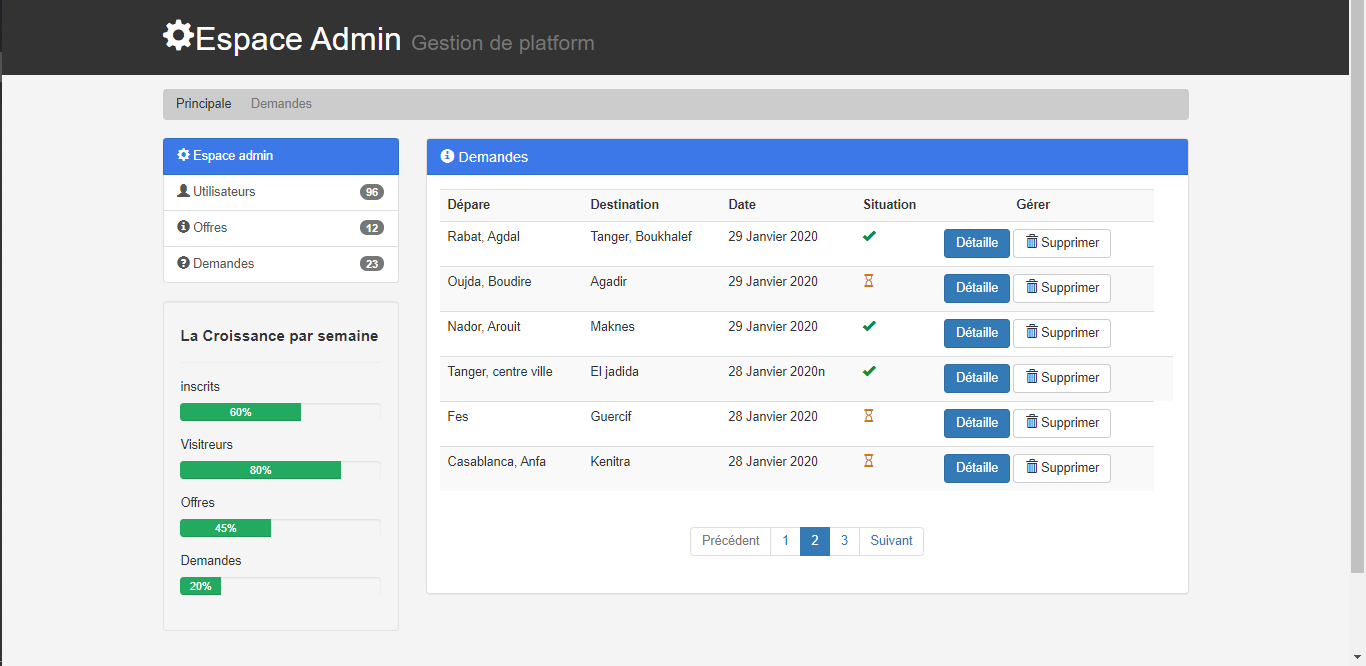
\includegraphics[height=8cm]{admin_demandes.png}
\end{center}
\caption[Espace admin]{Espace admin}
\end{figure}
\begin{figure}[!ht]
\begin{center}
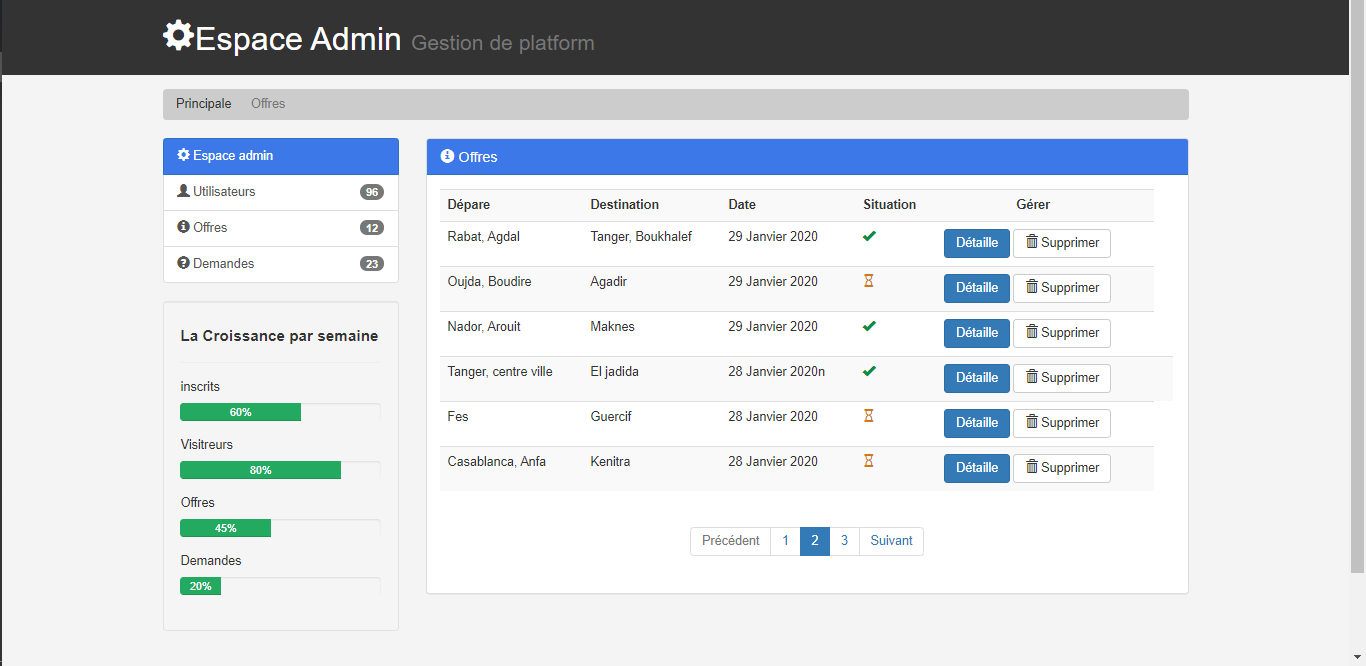
\includegraphics[height=8cm]{admin_offres.png}
\end{center}
\caption[Espace admin]{Espace admin}
\end{figure}

\cleardoublepage

\section{Problèmes rencontrés durant le projet}
\begin{spacing}{2}
\par 
Durant la réalisation du projet, nous avons rencontré des problèmes dont les unes sont plus graves que les autres. Nous avons pu trouver des solutions à certaines problèmes mais il restait des problèmes sans solution qui ont retardé l'avancement de notre projet. Je les cite comme suit :
\begin{itemize}
\item[•] \textbf{Implémentation des API :} nous avons trouvé du mal à introduire les API surtout celles du Google Maps et du Facebook. Des contraintes de paiement et de restrictions ont été imposées, ce qui a limité les fonctionnalités de notre projet : nous avons réussi à implémenter l'API du Facebook mais très limité. 
\item[•] \textbf{Implémentation du Chat Bot:} le déploiement du Chat Bot dans notre application n'a pas été possible parce que la dependency correspondante au Chat Bot n'a pas été identifiée correctement.
\item[•] \textbf{Upload des images dans les profils des utilisateurs :} problème de chargement de l'image au premier accès à l'espace de l'utilisateur.
\item[•] \textbf{Différentes configurations sur un le même projet:} nous avons adopté les solutions cherchées sur Internet mais ça n'a pas marché. 
\end{itemize} 

\par
Pour toute référence et détails sur un problème , veuillez accéder à notre projet sur GitHub dans la sections Issues. 
\begin{figure}[!ht]
\begin{center}
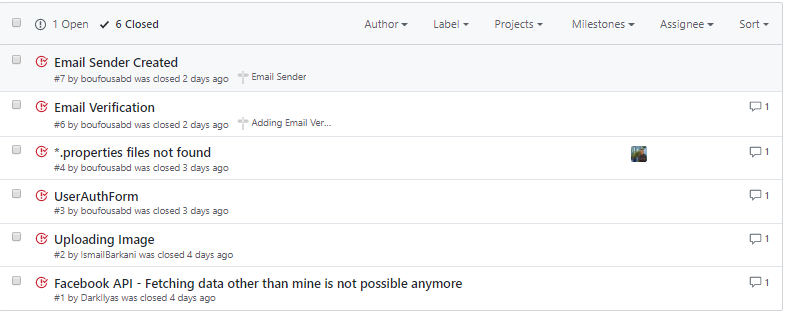
\includegraphics[height=6cm]{issues.png}
\end{center}
\caption[Section Issues du projet]{Section Issues du projet\protect\footnotemark}
\end{figure}
\footnotetext{lien vers la section Issues du projet https://github.com/ENSIAS-MEH/Wasselni--Platforme-de-covoiturage-JEE-/issues } 

\end{spacing}

\end{spacing}

\end{document}